\documentclass[10pt]{article}

%math
\usepackage{amsmath}
\usepackage{amssymb}
\usepackage{mathtools}
%logic
\usepackage{pgffor}
\usepackage{ifthen}
%science
\usepackage{siunitx}
\usepackage[version=4]{mhchem}
%language
\usepackage[english]{babel}
%formatting
\usepackage[a4paper, portrait, margin=1in]{geometry}
\usepackage[small]{titlesec}
\usepackage[hidelinks]{hyperref}
\usepackage{parskip}
\usepackage[doublespacing]{setspace}
\usepackage{layouts}
%images and plots
\usepackage{graphicx}
\usepackage[justification=centering]{caption}
\usepackage{subcaption}
\usepackage{float}
\usepackage{pgf}
\usepackage{import}
\usepackage{tikz}
\usetikzlibrary{arrows.meta, decorations.pathmorphing}
\usepackage{jsonparse}
%tables
\usepackage{booktabs}
\usepackage{makecell}
%citation, quatation and lists
\usepackage[
	style=numeric,
	maxcitenames=2,
	sorting=none,
	doi=false,
	url=false,
	isbn=false,
	eprint=false,
	urldate=long
]{biblatex}
\usepackage[inline]{enumitem}
\usepackage[noabbrev, nameinlink]{cleveref}
\usepackage{csquotes}
\usepackage[nottoc]{tocbibind}
\usepackage{acro}

%setup plugins
\addbibresource{literature.bib}

\captionsetup{justification=centering}
\hypersetup{colorlinks=true, linkcolor=blue, urlcolor=blue}

\DeclareSIUnit\angstrom{\text{Å}}
\DeclareSIUnit\bar{bar}
\sisetup{ range-phrase = { to } }

% Custom \citeauthoryear command with hyperref -> Rost et al. (2019)
\DeclareCiteCommand{\citeauthoryear}
{\boolfalse{citetracker}%
\boolfalse{pagetracker}%
\usebibmacro{prenote}}
{\ifciteindex {\indexnames{labelname}\indexfield{year}} {}%
\printtext[bibhyperref]{%
\printnames{labelname}%
\setunit{\addspace}%
\printtext{(}%
\printfield{year}%
\printtext{)}}}
{\multicitedelim}
{\usebibmacro{postnote}}

%  setup custom commands
\newcommand{\imcite}[2][]{From~\cite[#1]{#2}.}
\newcommand{\imcitetwo}[2][]{Based on~\cite[#1]{#2}.}
\newcommand{\integral}[4]{\int_{#1}^{#2} #3 \mathrm{d} #4}
\newcommand{\derivative}[2]{\frac{\mathrm{d}}{\mathrm{d} #1} #2}

% acronyms used throughout this report
\DeclareAcronym{dhs}{ short = DHS, long = double heterostructure }
\DeclareAcronym{sch}{ short = SCH, long = separate-confinement heterostructure }
\DeclareAcronym{qw}{ short = QW, long = quantum well }

\newcommand{\CellWithForceBreak}[2][c]{
\begin{tabular}[#1]{@{}c@{}}
	#2
\end{tabular}}

% Document
\begin{document}
	\pagenumbering{arabic}
	% !TEX root = ../main.tex
\begin{centering}
	\huge Semiconductor Physics Laboratory \RN{2}\\
	\LARGE B7: Laser Diodes\\
	\vspace{0.35cm}
	\normalsize Simon Legtenborg, 3773994 \\
	\normalsize Tim Düvel, 3785422 \\
	\normalsize Experiment conducted on 07/10/26 \\
	\vspace{1cm}
\end{centering}

	\setcounter{tocdepth}{2}
	\begin{singlespace}
		\hypersetup{linkcolor=black}
		\tableofcontents
	\end{singlespace}
	\clearpage
	% !TEX root = ../main.tex
\section{Introduction}
\label{sec:introduction}

Semiconductor lasers are an outstanding result of applied research in the 20th century.
The first semiconductor laser was built with $\ce{GaAs}$ in 1962. Decades of
continuous material and device optimization have made laser diodes standard
optoelectronic components. These advanced devices are used in modern technology,
primarily in fiber-optic communication and optical data storage.

A semiconductor laser uses radiative transitions of electrons between the
valence band and the conduction band to generate photons. It contains a zone in which
the light intensity increases if it is pumped sufficiently. This amplifying zone
is called the gain region. The light wave bounces back and forth in an optical cavity,
thereby constraining the available wavelengths. The proportion of light exiting the
device resembles a laser beam.

Semiconductor lasers can be made using a forward-biased PN Diode. The effect is
caused by interband transitions, therefore, the emission wavelength is
determined primarily by the band gap of the material.

Semiconductor materials with a direct band gap are suitable for laser
applications in different spectral ranges. Different material systems and their corresponding
wavelengths are displayed in \cref{fig:laser_materials}. 

\begin{figure}[H]
	\centering
	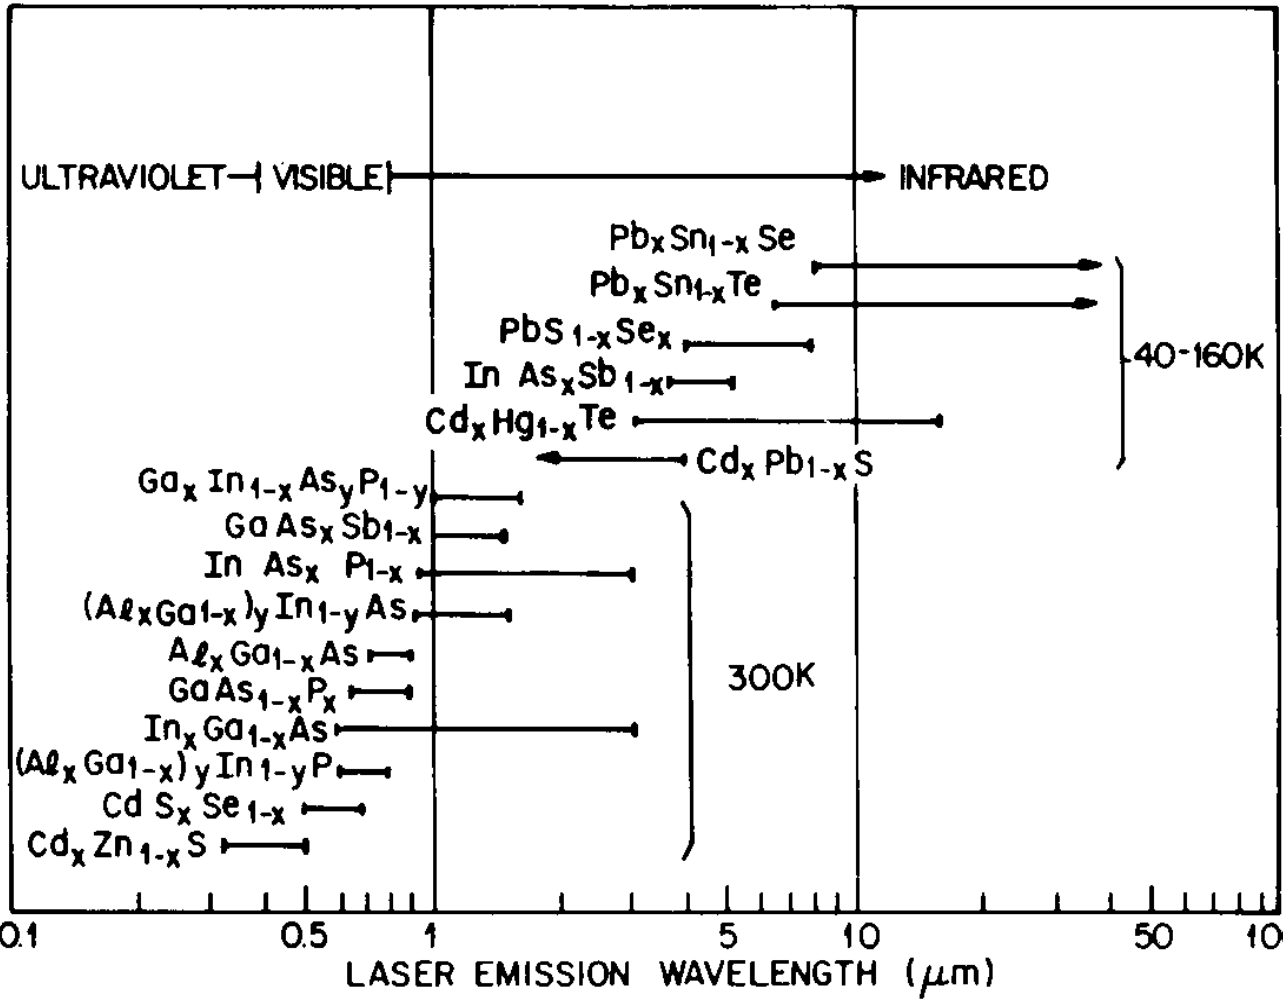
\includegraphics[width=0.5\linewidth]{../assets/laser_materials.png}
	\caption{Laser emission wavelength ranges for different semiconductor material
	systems, separated into room-temperature (\qty{300}{\kelvin}) and low-temperature
	(\qtyrange{40}{60}{\kelvin}{40}{unit}). \imcite{sze_physics_2021}. }
	\label{fig:laser_materials}
\end{figure}
	% !TEX root = ../main.tex
\section{Semiconductor Foundations}
\label{sec:semiconductor_foundations}

Before the working principle of a laser diode can be discussed in detail, preliminary
knowledge about carrier and photon statistics is required. Furthermore, the diode
current-voltage characteristics are discussed in this section, as they are not the
main focus of this laboratory course.

\subsection{Carrier Statistics}
\label{sec:carrier_statistics}

In thermal equilibrium, the probability that an electronic state of energy $E$ is
occupied is given by the Fermi-Dirac distribution, with the Fermi level $E_{\mathrm{F}}$,
the Boltzmann constant $k_{\mathrm{B}}$ and the temperature $T$:
\begin{equation}
	f(E)=\frac{1}{1+\exp\left[(E-E_{\mathrm{F}})/k_{\mathrm{B}}T\right]}.
\end{equation}

However, under non-equilibrium conditions (e.g., under an applied external voltage),
electron and hole densities can take arbitrary values in principle. In many
practically relevant cases, the carriers within each band are locally in thermal equilibrium
among themselves, but not with other bands. Instead of a constant Fermi level,
electron and hole densities are described locally at position $\mathbf{r}$ using quasi-Fermi levels
$F_{\mathrm{n}}(\mathbf{r})$ and $F_{\mathrm{p}}(\mathbf{r})$, and the respective
occupation probabilities are given by:
\begin{equation}
	f_{\mathrm{n}}(E, \mathbf{r}) = \frac{1}{1+\exp\left[(E-F_{\mathrm{n}}(\mathbf{r}))/k_{\mathrm{B}}T\right]}, \qquad
	f_{\mathrm{p}}(E, \mathbf{r}) = \frac{1}{1+\exp\left[(F_{\mathrm{p}}(\mathbf{r})-E)/k_{\mathrm{B}}T\right]}.
	\label{eq:occupation_probabilities}
\end{equation}
The electron density $n(\mathbf{r})$ and the hole density $p(\mathbf{r})$ are obtained
by integrating the product of the occupation probability and the density of states
$D_{\mathrm{n}}(E)$ or $D_{\mathrm{p}}(E)$ of the electrons or holes, respectively.
The integration runs over the conduction band above its edge $E_{\mathrm{C}}$ and
over the valence band below its edge $E_{\mathrm{V}}$:
\begin{equation}
	n(\mathbf{r}) = \int_{E_{\mathrm{C}}}^{\infty}D_{\mathrm{n}}(E)\, f_{\mathrm{n}}
	(E,\mathbf{r}) \,\mathrm{d}E, \qquad p(\mathbf{r}) = \int_{-\infty}^{E_{\mathrm{V}}}
	D_{\mathrm{p}}(E)\, f_{\mathrm{p}}(E,\mathbf{r}) \,\mathrm{d}E.
\end{equation}
Using the Boltzmann approximation, the integrals can be evaluated analytically, resulting
in the following expressions with the intrinsic carrier density $n_{\mathrm{i}}$ and the
intrinsic Fermi level $E_{\mathrm{i}}(\mathbf{r})$:
\begin{equation}
	n(\mathbf{r}) = n_{\mathrm{i}}\exp\left[\frac{F_{\mathrm{n}}(\mathbf{r}) - E_{\mathrm{i}}(\mathbf{r})}{k_{\mathrm{B}}T}\right], \qquad
	p(\mathbf{r}) = n_{\mathrm{i}}\exp\left[\frac{E_{\mathrm{i}}(\mathbf{r}) - F_{\mathrm{p}}(\mathbf{r})}{k_{\mathrm{B}}T}\right].
\end{equation}

The splitting $\Delta F(\mathbf{r})=F_{\mathrm{n}}(\mathbf{r})-F_{\mathrm{p}}(\mathbf{r}
)$ is a local quantity: it fixes the carrier product $np$ at each position. The applied
voltage $V$ is a global quantity: it fixes the difference between the quasi-Fermi
levels of the two contacts, with $V>0$ for forward bias and the elementary charge $e$:
\begin{equation}
	eV=F_{\mathrm{n}}(\text{n-contact})-F_{\mathrm{p}}(\text{p-contact}).
\end{equation}

\subsection{Joint Density of States}
\label{sec:band_structure}

Near the zone center of a direct semiconductor, the conduction and valence bands
can often be approximated by parabolic functions:
\begin{equation}
	E_{\mathrm{c}}(k)=E_{\mathrm{C}}+\frac{\hbar^{2}k^{2}}{2m_{\mathrm{e}}^{*}},\qquad
	E_{\mathrm{v}}(k)=E_{\mathrm{V}}-\frac{\hbar^{2}k^{2}}{2m_{\mathrm{h}}^{*}},\qquad
	E_{\mathrm{g}}=E_{\mathrm{C}}-E_{\mathrm{V}}.
	\label{eq:band_dispersion}
\end{equation}
Here, $k$ is the magnitude of the wavevector, $\hbar$ the reduced Planck constant,
$m_{\mathrm{e}}^{*}$ and $m_{\mathrm{h}}^{*}$ the effective masses of electrons and
holes, $E_{\mathrm{C}}$ and $E_{\mathrm{V}}$ the conduction band minimum and the
valence band maximum, and $E_{\mathrm{g}}$ the band gap. The energy difference
$E_{\mathrm{cv}}(k)$ between the two bands can be stated using the reduced mass
$m_{\mathrm{r}}$:
\begin{equation}
	E_{\mathrm{cv}}(k)=E_{\mathrm{c}}(k)-E_{\mathrm{v}}(k)=E_{\mathrm{g}}+\frac{\hbar^{2}k^{2}}{2m_{\mathrm{r}}}
	,\qquad \frac{1}{m_{\mathrm{r}}}=\frac{1}{m_{\mathrm{e}}^{*}}+\frac{1}{m_{\mathrm{h}}^{*}}
	.
	\label{eq:parabolic_bands}
\end{equation}

An optical transition in a semiconductor conserves energy as well as momentum of the
participating electron and photon. As the photon wavevector is small compared to
the extent of the Brillouin Zone, transitions can be approximated as vertical in $\mathbf{k}$-space.

The rate of optical transitions at energy $E$ depends on how many pairs of electronic
states are separated by exactly this energy. The number of available transitions
per unit volume and per energy is called the joint density of states
$D_{\mathrm{j}}(E)$ and is defined as:
\begin{equation}
	\text{\setstretch{1}
	\begin{tabular}{@{}c@{}}
		number of transitions per unit volume \\
		with energy in $[E_{0}, E_{1}]$
	\end{tabular}}= \int_{E_{0}}^{E_{1}}D_{\mathrm{j}}(E) \, \mathrm{d}E.
\end{equation}
Analogous to the electronic density of states, $D_{\mathrm{j}}$ can be defined
by counting the $\mathbf{k}$-states on the surface $S(\hbar\omega)$ of constant
transition energy $E_{\mathrm{cv}}(\mathbf{k})=\hbar\omega$, where $\omega$ is the
angular frequency of the photon:
\begin{equation}
	D_{\mathrm{j}}(\hbar \omega)= \frac{2}{V}\int_{S(\hbar \omega)}\frac{\mathrm{d}^{2}S}{\left(
	\frac{2\pi}{L}\right)^{3}\lvert \nabla_{\mathbf{k}}E_{\mathrm{cv}}(\mathbf{k}) \rvert
	}.
	\label{eq:joint_dos_surface}
\end{equation}
The factor 2 counts the two spin orientations, and $V=L^{3}$ is the volume of the
periodic boundary box with edge length $L$. By using the parabolic band approximation,
this integral can be solved analytically, with the Heaviside step function $\Theta$:
\begin{equation}
	D_{\mathrm{j}}(\hbar\omega)=\frac{1}{2\pi^{2}}\left(\frac{2m_{\mathrm{r}}}{\hbar^{2}}
	\right)^{3/2}\sqrt{\hbar\omega-E_{\mathrm{g}}}\;\Theta(\hbar\omega-E_{\mathrm{g}}
	).
\end{equation}

\subsection{Photon Mode Density and Statistics}
\label{sec:photons}

The allowed states of a photon field can be constructed using periodic boundary conditions
for the photon wave $\psi_{\mathbf{k}}$. These conditions result in a finite
set of allowed $\mathbf{k}$ vectors, with integers $l$, $m$, $n$ and the edge length
$L$ of the periodic boundary box:
\begin{equation}
	k_{x}=l \frac{2\pi}{L}, \quad k_{y}=m \frac{2\pi}{L}, \quad k_{z}=n \frac{2\pi}{L}
	.
\end{equation}

Analogous to the electronic density of states, the photon mode density of states $N
(E)$ can be constructed by counting the number of available states with energy $E$.
As the periodic boundary conditions lead to the same density of states in
$\mathbf{k}$-space as for the electrons, \cref{eq:joint_dos_surface} can be used
analogously, with a polarization factor of 2 (two transverse polarization states)
instead of the spin factor of 2. Substituting the photon energy relation
$E(\mathbf{k})=\hbar \lvert \mathbf{k}\rvert c /n_{\mathrm{r}}$ with the vacuum speed
of light $c$ for a dispersion-free medium, i.e. a constant refractive index
$n_{\mathrm{r}}$, the integral simplifies to:
\begin{equation}
	N(E)=\frac{n_{\mathrm{r}}^{3}E^{2}}{\pi^{2}\hbar^{3}c^{3}}.
\end{equation}

The spectral photon density $S(E)$, i.e. the number of photons per unit volume and
unit energy at energy $E$, is the product of the mode density $N(E)$ and the average
photon occupation number per mode $n_{\mathrm{ph}}(E)$:
\begin{equation}
	S(E)=N(E) \cdot n_{\mathrm{ph}}(E).
\end{equation}

As photons are bosonic particles, they obey the Bose-Einstein Statistics. In thermal
equilibrium with the lattice at temperature $T$, the occupation number $n_{\mathrm{ph}}$
per mode with energy $E$ is therefore given by:
\begin{equation}
	n_{\mathrm{ph}}(E)=\frac{1}{\exp\left( \dfrac{E}{k_{\mathrm{B}}T} \right) - 1}.
\end{equation}

\subsection{Diode Current-Voltage Characteristics}
\label{sec:carrier_injection}

The current-voltage characteristic of an ideal diode is described by the
Shockley equation for the current $I$, with the saturation current $I_{0}$ and the
voltage $V_{\mathrm{a}}$ across the junction:
\begin{equation}
	I = I_{0}\left[ \exp\left(\frac{eV_{\mathrm{a}}}{k_{\mathrm{B}}T}\right) - 1 \right
	].
\end{equation}
In the forward direction ($V_{\mathrm{a}}> 0$), the current increases
exponentially with the voltage, while in the reverse direction ($V_{\mathrm{a}}< 0$)
it saturates at the small reverse current $-I_{0}$. Real diodes are often
described by replacing $k_{\mathrm{B}}T$ with $n_{\mathrm{id}}k_{\mathrm{B}}T$, where
the ideality factor $n_{\mathrm{id}}$ usually lies between 1 and 2.

In a real diode, part of the applied voltage $V$ drops across the series resistance
$R_{\mathrm{s}}$ of the semiconductor bulk and the contacts. Only the remaining
voltage $V_{\mathrm{a}}= V - IR_{\mathrm{s}}$ is present at the junction, so the characteristic
becomes:
\begin{equation}
	I = I_{0}\left[\exp\left(\frac{e(V - IR_{\mathrm{s}})}{n_{\mathrm{id}} k_{\mathrm{B}}T}\right) -
	1\right].
	\label{eq:schockley_real}
\end{equation}
	% !TEX root = ../main.tex
\section{Optical Transitions: Absorption, Stimulated and Spontaneous Emission}
\label{sec:optical_transitions}

\begin{figure}[H]
	\centering
	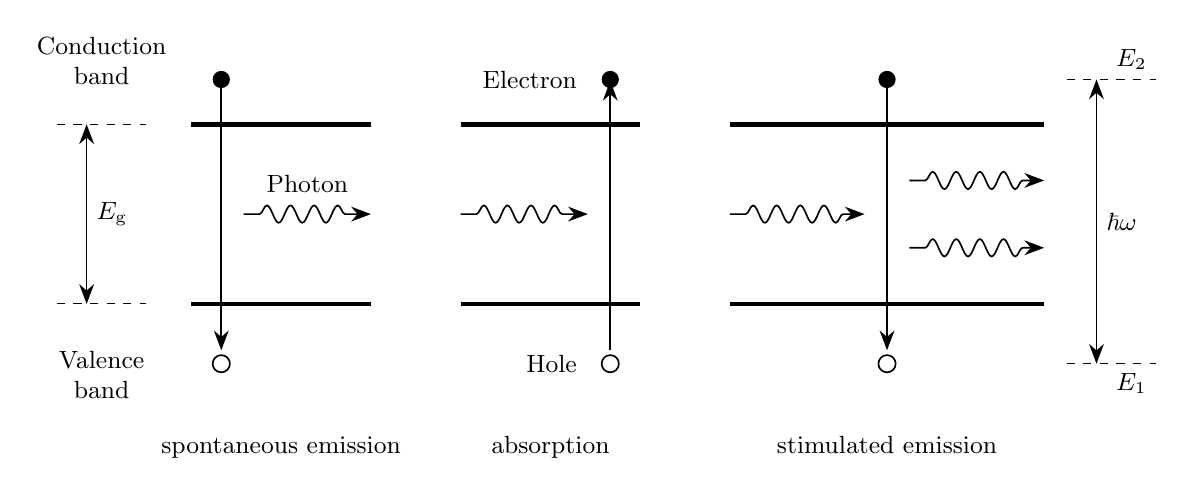
\begin{tikzpicture}[
		x=1cm,
		y=1cm,
		scale=0.95,
		every node/.style={font=\small\setstretch{1}},
		band/.style={line width=1.6pt},
		level/.style={dashed},
		transition/.style={-{Stealth[length=2.5mm]}, semithick},
		photon/.style={-{Stealth[length=2.5mm]}, semithick, decorate, decoration={snake, amplitude=1.1mm, segment length=3mm, pre length=2mm, post length=2.5mm}},
		electron/.style={circle, fill, inner sep=2.2pt},
		hole/.style={circle, draw, semithick, fill=white, inner sep=2.2pt},
	]
		% spontaneous emission
		\draw[level] (0.1, 2.4) -- (1.3, 2.4);
		\draw[level] (0.1, 0) -- (1.3, 0);
		\draw[{Stealth[length=2.5mm]}-{Stealth[length=2.5mm]}, semithick]
			(0.5, 0) --
			node[right] {$E_{\mathrm{g}}$}
			(0.5, 2.4);
		\draw[band] (1.9, 2.4) -- (4.3, 2.4);
		\draw[band] (1.9, 0) -- (4.3, 0);
		\draw[transition] (2.3, 3.0) -- (2.3, -0.62);
		\node[electron] at (2.3, 3.0) {};
		\node[hole] at (2.3, -0.8) {};
		\draw[photon] (2.6, 1.2) -- node[above=1.5mm] {Photon} (4.3, 1.2);
		\node[align=center] at (0.7, 3.25) {Conduction\\band};
		\node[align=center] at (0.7, -0.95) {Valence\\band};
		\node[anchor=base] at (3.1, -2.0) {spontaneous emission};

		% absorption
		\draw[band] (5.5, 2.4) -- (7.9, 2.4);
		\draw[band] (5.5, 0) -- (7.9, 0);
		\draw[transition] (7.5, -0.62) -- (7.5, 2.98);
		\node[electron] at (7.5, 3.0) {};
		\node[hole] at (7.5, -0.8) {};
		\draw[photon] (5.5, 1.2) -- (7.2, 1.2);
		\node[left=3mm] at (7.5, 3.0) {Electron};
		\node[left=3mm] at (7.5, -0.8) {Hole};
		\node[anchor=base] at (6.7, -2.0) {absorption};

		% stimulated emission
		\draw[band] (9.1, 2.4) -- (13.3, 2.4);
		\draw[band] (9.1, 0) -- (13.3, 0);
		\draw[transition] (11.2, 3.0) -- (11.2, -0.62);
		\node[electron] at (11.2, 3.0) {};
		\node[hole] at (11.2, -0.8) {};
		\draw[photon] (9.1, 1.2) -- (10.9, 1.2);
		\draw[photon] (11.5, 1.65) -- (13.3, 1.65);
		\draw[photon] (11.5, 0.75) -- (13.3, 0.75);
		\node[anchor=base] at (11.2, -2.0) {stimulated emission};

		% transition energy
		\draw[level] (13.6, 3.0) -- (14.8, 3.0) node[above left] {$E_{2}$};
		\draw[level] (13.6, -0.8) -- (14.8, -0.8) node[below left] {$E_{1}$};
		\draw[{Stealth[length=2.5mm]}-{Stealth[length=2.5mm]}, semithick]
			(14.0, -0.8) --
			node[right] {$\hbar\omega$}
			(14.0, 3.0);
	\end{tikzpicture}
	\caption{Band diagrams of the optical transitions between the conduction and
	the valence band: spontaneous emission, absorption and stimulated emission. \imcite{benndorf_semiconductor_nodate}}
	\label{fig:optical_transitions}
\end{figure}

An incoming photon induces a perturbation of the electronic system of the
semiconductor, which may result in the generation of an electron-hole pair. This
process is called absorption. For this electronic excitation to occur, the
energy $\hbar \omega$ of the incoming photon must be at least the band gap
energy $E_{\mathrm{g}}$.

An incoming photon induces a perturbation of the electronic system of the
semiconductor, which may result in a radiative recombination of an electron-hole pair.
The incoming and the generated photon are coherent, i.e., they share the same direction,
phase, frequency and polarization. The process requires an electron in the
conduction band and a hole in the valence band and is called stimulated emission.

Without any incoming photon, an electron in the conduction band can recombine radiatively
with a hole in the valence band. The emitted photons have random directions and
phases, so the resulting light is incoherent. This process is called spontaneous
emission. All three processes are depicted in \cref{fig:optical_transitions}.

\subsection{Mathematical Description}
\label{sec:mathematical_description}

\begin{table}
	\centering
	\begin{tabular}{lll}
		\toprule Process            & $i$             & $\Phi^{(i)}$                           \\
		\midrule absorption (gross) & $\mathrm{abs}$  & $(1-f_{\mathrm{n}})(1-f_{\mathrm{p}})$ \\
		stimulated emission (gross) & $\mathrm{stim}$ & $f_{\mathrm{n}}f_{\mathrm{p}}$         \\
		spontaneous emission        & $\mathrm{spon}$ & $f_{\mathrm{n}}f_{\mathrm{p}}$         \\
		\bottomrule
	\end{tabular}
	\caption{Occupation factors for absorption, stimulated and spontaneous emission.}
	\label{tab:occupation_factors}
\end{table}

Absorption, stimulated emission and spontaneous emission can all be described
using a single formula based on Fermi's Golden Rule. The rate coefficients $r^{(i)}$,
i.e., the rates normalized to one photon per mode, are given by:
\begin{equation}
	r^{(i)}(\hbar\omega)=P(\hbar\omega)\sum_{\mathbf{k}_{\mathrm{p}},\mathbf{k}_{\mathrm{n}}}
	\frac{2}{V}\lvert\hat e\cdot\mathbf{p}_{\mathrm{cv}}(\mathbf{k}_{\mathrm{p}},\mathbf{k}
	_{\mathrm{n}})\rvert^{2}\,\delta\big(E_{\mathrm{c}}(\mathbf{k}_{\mathrm{n}})-E_{\mathrm{v}}
	(\mathbf{k}_{\mathrm{p}})-\hbar\omega\big)\;\Phi^{(i)}\label{eq:universal_rate_equation}
\end{equation}
The factor $2/V$ counts both spin orientations per unit volume. $\Phi^{(i)}$ is the
occupation factor of process $i$, eludicated in \cref{tab:occupation_factors}. The
occupation factors depend on $E_{\mathrm{c}}(\mathbf{k}_{\mathrm{n}})$ and $E_{\mathrm{v}}
(\mathbf{k}_{\mathrm{p}})$ individually (via $f_{\mathrm{n}}$ and
$f_{\mathrm{p}}$), not only on their difference. The remaining prefactors are given
by:
\begin{equation}
	P(\hbar\omega)=\frac{n_{\mathrm{r}}^{2}(\hbar\omega)^{2}}{\pi^{2}\hbar^{3}c^{2}}
	\,C_{0}(\hbar\omega),\qquad C_{0}(\hbar\omega)=\frac{\pi e^{2}\hbar}{n_{\mathrm{r}}c\,\epsilon_{0}m_{0}^{2}\,\hbar\omega}
	\quad\Rightarrow\quad P(\hbar\omega)=\frac{n_{\mathrm{r}}e^{2}}{\pi\hbar^{2}c^{3}\epsilon_{0}m_{0}^{2}}
	\;\hbar\omega.
\end{equation}

Note that $r^{(i)}$ are normalized to one photon per mode and can therefore be regarded
as material-specific quantities. However, the actual absorption and stimulated emission
rates depend on the photon occupation number $n_{\mathrm{ph}}$:
\begin{equation}
	R^{\mathrm{abs}}= n_{\mathrm{ph}}\cdot r^{\mathrm{abs}}, \qquad R^{\mathrm{stim}}
	= n_{\mathrm{ph}}\cdot r^{\mathrm{stim}}, \qquad R^{\mathrm{spon}}=r^{\mathrm{spon}}
	.
\end{equation}

\subsection{Analytical Line Shape}
\label{sec:line_shape}

Under three additional assumptions, the universal emission and absorption rates yield
an analytical line shape:

\begin{enumerate}[label=(\roman{*}), ref=(\roman{*})]
	\item \label{ass:k_selection} Vertical transitions ($\mathbf{k}$-selection):
		$\lvert \hat{e}\cdot \mathbf{p}_{\mathrm{cv}}(\mathbf{k}_{\mathrm{p}},\mathbf{k}
		_{\mathrm{n}}) \rvert^{2}=\lvert \hat{e}\cdot \mathbf{p}_{\mathrm{cv}}\rvert^{2}
		\, \delta_{\mathbf{k}_{\mathrm{p}} \mathbf{k}_{\mathrm{n}}}$,

	\item \label{ass:const_matrix} a constant matrix element:
		$\lvert\hat e\cdot\mathbf{p}_{\mathrm{cv}}\rvert^{2}=\mathrm{const.}$,

	\item \label{ass:parabolic} parabolic bands, see \cref{eq:parabolic_bands}.
\end{enumerate}

Substituting assumptions~\ref{ass:k_selection} and~\ref{ass:const_matrix} into
\cref{eq:universal_rate_equation} yields:
\begin{equation}
	r^{(i)}(\hbar\omega)= P(\hbar\omega)\, \frac{2}{V}\lvert\hat e\cdot\mathbf{p}_{\mathrm{cv}}
	\rvert^{2}\sum_{\mathbf{k}}\delta\big(E_{\mathrm{cv}}(\mathbf{k})-\hbar\omega\big
	)\;\Phi^{(i)}(\mathbf{k})
\end{equation}

The sum is converted to an integral with the density of $\mathbf{k}$-states
$V/(2 \pi)^{3}$.
\begin{equation}
	\quad r^{(i)}(\hbar\omega)= P(\hbar\omega)\,\lvert\hat e\cdot\mathbf{p}_{\mathrm{cv}}
	\rvert^{2}\, \frac{2}{(2\pi)^{3}}\int \delta\big(E_{\mathrm{cv}}(\mathbf{k})-\hbar
	\omega\big)\;\Phi^{(i)}(\mathbf{k})\,\mathrm{d}\mathbf{k}
\end{equation}

For the isotropic bands of assumption~\ref{ass:parabolic}, the integrand depends only
on $k=\lvert\mathbf{k}\rvert$, so the angular integration can be performed
directly and $\mathrm{d}\mathbf{k}\to4\pi k^{2}\,\mathrm{d}k$:
\begin{equation}
	r^{(i)}(\hbar\omega)= P(\hbar\omega)\,\lvert\hat e\cdot\mathbf{p}_{\mathrm{cv}}
	\rvert^{2}\, \frac{1}{\pi^{2}}\int_{0}^{\infty}k^{2}\,\delta\big(E_{\mathrm{cv}}
	(k)-\hbar\omega\big)\;\Phi^{(i)}(k)\,\mathrm{d}k
\end{equation}

Changing the integration variable from $k$ to $E_{\mathrm{cv}}$ with the
parabolic dispersion of assumption~\ref{ass:parabolic} yields: With $k=k(E_{\mathrm{cv}}
)$, the occupation factor becomes $\Phi^{(i)}\big(k(E_{\mathrm{cv}})\big)$, and the
delta distribution can be evaluated directly. It fixes
$E_{\mathrm{cv}}(k_{0})=\hbar\omega$, i.e., $k=k_{0}$ with $k_{0}$ the magnitude of
the wavevector at photon energy $\hbar\omega$, so that $\Phi^{(i)}$ is evaluated
at $k_{0}$:
\begin{align}
	r^{(i)}(\hbar\omega) & = P(\hbar\omega)\,\lvert\hat e\cdot\mathbf{p}_{\mathrm{cv}}\rvert^{2}\, \frac{1}{2\pi^{2}}\left(\frac{2m_{\mathrm{r}}}{\hbar^{2}}\right)^{3/2}\int_{E_{\mathrm{g}}}^{\infty}\sqrt{E_{\mathrm{cv}}-E_{\mathrm{g}}}\;\delta(E_{\mathrm{cv}}-\hbar\omega)\;\Phi^{(i)}\big(k(E_{\mathrm{cv}})\big)\,\mathrm{d}E_{\mathrm{cv}} \\
	                     & = P(\hbar\omega)\,\lvert\hat e\cdot\mathbf{p}_{\mathrm{cv}}\rvert^{2}\, \underbrace{\frac{1}{2\pi^{2}}\left(\frac{2m_{\mathrm{r}}}{\hbar^{2}}\right)^{3/2}\sqrt{\hbar\omega-E_{\mathrm{g}}}\;\Theta(\hbar\omega-E_{\mathrm{g}})}_{D_{\mathrm{j}}(\hbar\omega)}\;\Phi^{(i)}(k_{0})
\end{align}

In this equation, $D_{\mathrm{j}}$ is the Joint Density of States (including
spin). With the energy zero at the valence-band maximum, $E_{\mathrm{c}}(k)=E_{\mathrm{g}}
+\frac{\hbar^{2}k^{2}}{2m_{\mathrm{e}}^{*}}$ and $E_{\mathrm{v}}(k)=-\frac{\hbar^{2}k^{2}}{2m_{\mathrm{h}}^{*}}$,
the occupation factors are evaluated at $k_{0}$, i.e., at the band energies $E_{\mathrm{c}}
(k_{0})$ and $E_{\mathrm{v}}(k_{0})$:
\begin{equation}
	k_{0}=\frac{\sqrt{2m_{\mathrm{r}}(\hbar\omega-E_{\mathrm{g}})}}{\hbar},\qquad E
	_{\mathrm{c}}(k_{0})=E_{\mathrm{g}}+\frac{m_{\mathrm{r}}}{m_{\mathrm{e}}^{*}}(\hbar
	\omega-E_{\mathrm{g}}),\qquad E_{\mathrm{v}}(k_{0})=-\frac{m_{\mathrm{r}}}{m_{\mathrm{h}}^{*}}
	(\hbar\omega-E_{\mathrm{g}})
\end{equation}

The absorption and emission line shape therefore starts at $E_{\mathrm{g}}$ and rises
as $\sqrt{\hbar\omega-E_{\mathrm{g}}}$, modulated by the prefactor
$P(\hbar \omega)$ and the occupation factor $\Phi^{(i)}(k_{0})$.

\subsection{Rate Ratios}
\label{sec:rate_ratios}

As absorption, stimulated emission and spontaneous emission follow from the same
general \cref{eq:universal_rate_equation}, their ratios can be calculated easily.

\subsubsection{Stimulated Emission vs Absorption}

Let $f_{\mathrm{n}}$ and $f_{\mathrm{p}}$ be the occupation probabilities of the
conduction band by electrons and of the valence band by holes, described by the Quasi
Fermi Levels $F_{\mathrm{n}}$ and $F_{\mathrm{p}}$ at the same temperature $T$:
\begin{align}
	\frac{1-f_{\mathrm{n}}}{f_{\mathrm{n}}}=\exp\left(\frac{E_{\mathrm{c}}-F_{\mathrm{n}}}{k_{\mathrm{B}}T}\right),\quad \frac{1-f_{\mathrm{p}}}{f_{\mathrm{p}}} & =\exp\left(\frac{F_{\mathrm{p}}-E_{\mathrm{v}}}{k_{\mathrm{B}}T}\right) \\
	\label{eq:f_n_identity}
\end{align}

The matrix elements cancel in the quotient of the absorption and stimulated-emission
rates, so that it equals the ratio of the occupation factors
$\Phi^{\mathrm{abs}}/\Phi^{\mathrm{stim}}$. Since the $\delta$-function fixes $E_{\mathrm{c}}
-E_{\mathrm{v}}=\hbar\omega$, it follows that:
\begin{equation}
	\frac{R^{\mathrm{abs}}}{R^{\mathrm{stim}}}=\frac{(1-f_{\mathrm{n}})(1-f_{\mathrm{p}})}{f_{\mathrm{n}}f_{\mathrm{p}}}
	=\exp\left[\frac{\hbar\omega-(F_{\mathrm{n}}-F_{\mathrm{p}})}{k_{\mathrm{B}}T}\right
	] \label{eq:abs_stim_rate}
\end{equation}

In thermal equilibrium, $F_{\mathrm{n}}=F_{\mathrm{p}}$ and $R^{\mathrm{abs}}> R^{\mathrm{stim}}$:
absorption always dominates. However, wave amplification is present if
$R^{\mathrm{stim}}> R^{\mathrm{abs}}$, i.e., if $F_{\mathrm{n}}-F_{\mathrm{p}}>\hbar
\omega$. Laser operation therefore requires a quasi-Fermi level separation that
exceeds the photon energy, which can only be achieved by strong carrier injection.

\subsubsection{Stimulated vs Spontaneous Emission}

The quotient of the stimulated and spontaneous emission rates equals the photon
occupation number $n_{\mathrm{ph}}$ per mode. With the mode density $N$ and the spectral
photon density $S=N\,n_{\mathrm{ph}}$, it follows that:
\begin{equation}
	\frac{R^{\mathrm{stim}}}{R^{\mathrm{spon}}}=n_{\mathrm{ph}}(\hbar \omega)=\frac{S(\hbar\omega)}{N(\hbar\omega)}
	=\frac{\pi^{2}\hbar^{3}c^{3}}{n_{\mathrm{r}}^{3}}\,\frac{S(\hbar\omega)}{(\hbar\omega)^{2}}
	\label{eq:stim_spon_rate}
\end{equation}

Since the ratio $R^{\mathrm{stim}}/R^{\mathrm{spon}}$ grows linearly with $S$, a high
photon density, achieved by waveguiding and a Fabry-Perot Resonator, shifts the balance
towards stimulated emission.

\subsubsection{Thermal Equilibrium}

In thermal equilibrium, the quasi-Fermi levels coincide,
$F_{\mathrm{n}}=F_{\mathrm{p}}$, and the photon occupation number follows the Bose-Einstein
distribution. Using \cref{eq:abs_stim_rate} and \cref{eq:stim_spon_rate}, the rates
satisfy:
\begin{align}
	\frac{R^{\mathrm{abs}}-R^{\mathrm{spon}}}{R^{\mathrm{stim}}} & =\exp\left( \frac{\hbar \omega- (F_{\mathrm{n}}-F_{\mathrm{p}})}{k_{\mathrm{B}}T}\right) - \frac{1}{n_{\mathrm{ph}}}                \\
	                                                             & =\exp\left( \frac{\hbar \omega}{k_{\mathrm{B}}T}\right) - \left[\exp\left( \frac{\hbar \omega}{k_{\mathrm{B}}T}\right) - 1\right]=1
\end{align}

Hence, absorption and total emission are in balance
$R^{\mathrm{abs}}=R^{\mathrm{stim}}+R^{\mathrm{spon}}$.

\subsection{Spontaneous Emission Line Shape}
\label{sec:spontaneous_emission}

Following \cref{sec:line_shape}, the spontaneous emission rate can be expressed
using the equilibrium absorption coefficient (see \cref{sec:absorption_coefficient_and_gain}),
the Photon Density of States $N(\hbar \omega)$ and the occupation probabilities $f
_{\mathrm{n}}$, $f_{\mathrm{p}}$.
\begin{equation}
	R^{\mathrm{spon}}(\hbar \omega)=N(\hbar\omega) \frac{c}{n_{\mathrm{r}}}\alpha_{0}
	(\hbar \omega) f_{\mathrm{n}}f_{\mathrm{p}}
\end{equation}

The occupation factors are evaluated in the Boltzmann approximation:
\begin{align}
	f_{\mathrm{n}}(E) & =\frac{1}{1+\exp\left( \frac{E-F_{\mathrm{n}}}{k_{\mathrm{B}}T} \right)}\simeq \exp\left( \frac{F_{\mathrm{n}}-E}{k_{\mathrm{B}}T}\right) \\
	f_{\mathrm{p}}(E) & =\frac{1}{1+\exp\left( \frac{F_{\mathrm{p}}-E}{k_{\mathrm{B}}T} \right)}\simeq \exp\left( \frac{E-F_{\mathrm{p}}}{k_{\mathrm{B}}T}\right)
\end{align}

The factors $f_{\mathrm{n}}$ and $f_{\mathrm{p}}$ are evaluated at the band
energies $E_{\mathrm{c}}(k_{0})$ and $E_{\mathrm{v}}(k_{0})$ of the transition, the
$\delta$-function fixes their difference to $E_{\mathrm{c}}(k_{0})-E_{\mathrm{v}}
(k_{0})=\hbar\omega$. The individual band energies therefore drop out of the
product and only the quasi-Fermi-level splitting
$\Delta F=F_{\mathrm{n}}-F_{\mathrm{p}}$ and the photon energy remain:
\begin{align}
	f_{\mathrm{n}}f_{\mathrm{p}} & \simeq \exp \left( \frac{F_{\mathrm{n}}-F_{\mathrm{p}}-\left(E_{\mathrm{c}}(k_{0})-E_{\mathrm{v}}(k_{0})\right)}{k_{\mathrm{B}}T}\right)=\exp \left( \frac{\Delta F -\hbar \omega}{k_{\mathrm{B}}T}\right) \\
	                             & =\exp\left( \frac{\Delta F-E_{\mathrm{g}}}{k_{\mathrm{B}}T}\right) \exp\left( -\frac{\hbar \omega-E_{\mathrm{g}}}{k_{\mathrm{B}}T}\right)
\end{align}

Inserting this into the rate gives the analytical spontaneous emission spectrum
(for $\hbar\omega>E_{\mathrm{g}}$), where $\Delta F$ only enters the amplitude:
\begin{equation}
	R^{\mathrm{spon}}(\hbar \omega)= N(\hbar\omega)\frac{c}{n_{\mathrm{r}}}\,\alpha
	_{0}(\hbar \omega)\,\exp\left( \frac{\Delta F-E_{\mathrm{g}}}{k_{\mathrm{B}}T}\right
	) \exp\left( -\frac{\hbar \omega-E_{\mathrm{g}}}{k_{\mathrm{B}}T}\right)
\end{equation}

With $N\propto(\hbar\omega)^{2}$ and $\alpha_{0}\propto\sqrt{\hbar\omega-E_{\mathrm{g}}}
\,/\,\hbar\omega$, the spectral shape follows:
\begin{equation}
	R^{\mathrm{spon}}(\hbar \omega)\propto \hbar\omega\,\sqrt{\hbar\omega-E_{\mathrm{g}}}
	\,\exp\left( -\frac{\hbar \omega-E_{\mathrm{g}}}{k_{\mathrm{B}}T}\right)
\end{equation}

\subsubsection{Measurable Quantities}

The number of photons emitted per volume and time with photon energies $E=\hbar\omega$
between $E_{1}$ and $E_{2}$ is:
\begin{equation}
	N(E_{1}, E_{2}) = \int_{E_1}^{E_2}R^{\mathrm{spon}}(E) \, \mathrm{d}E
\end{equation}

Weighting each photon by its energy gives the spectral power density $p_{E}(E)=E\,
R^{\mathrm{spon}}(E)$ and the emitted optical power per volume:
\begin{equation}
	P(E_{1}, E_{2})=\int_{E_1}^{E_2}p_{E}(E) \, \mathrm{d}E = \int_{E_1}^{E_2}E \, R
	^{\mathrm{spon}}(E) \, \mathrm{d}E
\end{equation}

The extra factor $E$ turns the factor $\hbar\omega$ of the rate into $(\hbar\omega
)^{2}$ in the power spectrum:
\begin{equation}
	p_{E}(E)\propto (\hbar\omega)^{2}\sqrt{ \hbar \omega-E_{\mathrm{g}}}\exp\left( -
	\frac{\hbar \omega-E_{\mathrm{g}}}{k_{\mathrm{B}}T}\right)
\end{equation}

Spectrometers usually resolve the emission in wavelength rather than in energy.
With $E=hc/\lambda$ (vacuum wavelength $\lambda$), the integral transforms as:
\begin{align}
	P(\lambda_{1}, \lambda_{2})           & =\int_{E_1}^{E_2}p_{E}(E)\,\mathrm{d}E=\int_{\lambda_2}^{\lambda_1}\underbrace{p_{E}\!\left(\frac{hc}{\lambda}\right)\frac{hc}{\lambda^{2}}}_{p_{\lambda}(\lambda)}\,\mathrm{d}\lambda                          \\
	\Rightarrow\quad p_{\lambda}(\lambda) & =p_{E}\!\left(\frac{hc}{\lambda}\right)\frac{hc}{\lambda^{2}}\propto\frac{1}{\lambda^{4}}\sqrt{\frac{hc}{\lambda}-E_{\mathrm{g}}}\,\exp\left( -\frac{\frac{hc}{\lambda}-E_{\mathrm{g}}}{k_{\mathrm{B}}T}\right)
\end{align}

A real detector measures the power within a finite bandwidth $\Delta\lambda=\lambda
_{1}-\lambda_{2}$. If $p_{\lambda}(\lambda)$ varies only slightly within this
interval, the integral can be approximated by the midpoint rule, and the
spectral power density at the center wavelength
$\lambda_{\mathrm{c}}=(\lambda_{1}+\lambda_{2})/2$ is approximately the measured
power divided by the interval width:
\begin{equation}
	P(\lambda_{1},\lambda_{2})\approx p_{\lambda}(\lambda_{\mathrm{c}})\,\Delta\lambda
	\quad\Rightarrow\quad p_{\lambda}(\lambda_{\mathrm{c}})\approx\frac{P(\lambda_{1},\lambda_{2})}{\Delta\lambda}
\end{equation}
	% !TEX root = ../main.tex
\section{Absorption Coefficient and Gain}
\label{sec:absorption_coefficient_and_gain}

The absorption coefficient $\alpha(\hbar \omega)$ is a fundamental material property,
used in the Lambert-Beer law $I(z)=I_{0}\exp(-\alpha z)$, which describes the decay
of the light intensity $I$ with the propagation distance $z$. The absorption
coefficient can be defined universally as:
\begin{equation}
	\alpha =\frac{\text{Number of photons absorbed per second per unit volume}}{\text{Number
	of injected photons per second per unit area}}.\label{eq:alpha}
\end{equation}
The numerator of \cref{eq:alpha} is the net absorption rate,
$R^{\mathrm{abs}}- R^{\mathrm{stim}}$ emission. Using its analytical form from \cref{sec:line_shape}
results in:
\begin{equation}
	R^{\mathrm{net}}=n_{\mathrm{ph}}(r^{\mathrm{abs}}-r^{\mathrm{stim}}) = n_{\mathrm{ph}}
	\, P(\hbar\omega) \lvert \hat{e}\cdot \mathbf{p}_{\mathrm{cv}}\rvert^{2}D_{\mathrm{j}}
	(\hbar\omega)\,(1-f_{\mathrm{n}}-f_{\mathrm{p}}).
\end{equation}
The denominator is the spectral photon flux, i.e. the number of injected photons
crossing a unit area per second per photon energy. This quantity is obtained from
the spectral photon density $S=n_{\mathrm{ph}}N$, travelling at the velocity
$c/n_{\mathrm{r}}$:
\begin{equation}
	F=n_{\mathrm{ph}}\cdot N \cdot \frac{c}{n_{\mathrm{r}}}= n_{\mathrm{ph}}\frac{n_{\mathrm{r}}^{2}\omega^{2}}{\pi^{2}\hbar
	c^{2}}.
\end{equation}

Dividing $R_{\mathrm{net}}$ by $F$ cancels $n_{\mathrm{ph}}$ and yields an
analytical expression for the absorption coefficient:
\begin{equation}
	\alpha(\hbar \omega)=\frac{R^{\mathrm{net}}}{F}=C_{0}\lvert \hat{e}\cdot\mathbf{p}
	_{\mathrm{cv}}\rvert^{2}D_{\mathrm{j}}(1-f_{\mathrm{n}}-f_{\mathrm{p}}). \label{eq:alpha_analytical}
\end{equation}

\subsection{Thermal Equilibrium}

In an undoped, unexcited semiconductor at low temperature ($k_{\mathrm{B}}T\ll E_{\mathrm{g}}$),
the valence band is full and the conduction band is empty,
$f_{\mathrm{n}}\approx 0$ and $f_{\mathrm{p}}\approx0$. The expression above then
reduces to the equilibrium absorption coefficient $\alpha_{0}$. The
approximation is valid if the considered energy interval is small:
\begin{equation}
	\alpha_{0}(\hbar \omega)=C_{0}\lvert \hat{e}\cdot \mathbf{p}_{\mathrm{cv}}\rvert
	^{2}D_{\mathrm{j}}\propto \frac{\sqrt{ \hbar \omega -E_{\mathrm{g}}}}{\hbar
	\omega}\simeq \sqrt{ \hbar \omega -E_{\mathrm{g}}}.
\end{equation}

\subsection{Non-Equilibrium and Bernard-Duraffourg Condition}

Away from equilibrium, $f_{\mathrm{n}}$ and $f_{\mathrm{p}}$ are governed by
separate quasi-Fermi levels, so $1-f_{\mathrm{n}}-f_{\mathrm{p}}$ can in principle
change sign. To this end, the occupation factor in \cref{eq:alpha_analytical} is rewritten
using \cref{eq:f_n_identity} with $E_{\mathrm{c}}(k_{0})-E_{\mathrm{v}}(k_{0})=\hbar
\omega$:
\begin{align}
	1-f_{\mathrm{n}}-f_{\mathrm{p}} & =(1-f_{\mathrm{n}})(1-f_{\mathrm{p}}) - f_{\mathrm{n}}f_{\mathrm{p}}=f_{\mathrm{n}}f_{\mathrm{p}}\left[ \frac{(1-f_{\mathrm{n}})(1-f_{\mathrm{p}})}{f_{\mathrm{n}}f_{\mathrm{p}}}- 1\right] \\
	                                & =f_{\mathrm{n}}f_{\mathrm{p}}\left[\exp\left( \frac{\hbar \omega -(F_{\mathrm{n}}-F_{\mathrm{p}})}{k_{\mathrm{B}}T}\right) -1\right]. \label{eq:f_n_identity_2}
\end{align}

Substituting \cref{eq:f_n_identity_2} into $\alpha(\hbar\omega)$ with the parabolic-band
joint density of states gives, with all energy-independent prefactors collected
in a constant:
\begin{equation}
	\alpha(\hbar \omega) = \underbrace{ \mathrm{const.} }_{ >0 }\; \underbrace{ \frac{\sqrt{
	\hbar \omega-E_{\mathrm{g}}}}{\hbar \omega} }_{ \hbar \omega >E_{\mathrm{g}} }\;
	\underbrace{ f_{\mathrm{n}} }_{ >0 }\; \underbrace{ f_{\mathrm{p}} }_{ >0 }\; \underbrace{
	\left[\exp\left( \frac{\hbar \omega -(F_{\mathrm{n}}-F_{\mathrm{p}})}{k_{\mathrm{B}}T}
	\right) -1\right] }_{ <0 \text{ if } \hbar \omega <F_{\mathrm{n}}-F_{\mathrm{p}}
	}.
\end{equation}
Only the bracket can change sign; every other factor in the expression is
positive. A negative value of the bracket corresponds to gain instead of absorption.
The bracket is negative exactly when
$\hbar\omega < F_{\mathrm{n}}-F_{\mathrm{p}}$; combined with the requirement $\hbar
\omega>E_{\mathrm{g}}$ for the transition to exist at all, this gives the
Bernard-Duraffourg condition: $F_{\mathrm{n}}-F_{\mathrm{p}}>\hbar \omega > E_{\mathrm{g}}$.

\subsection{Gain}

The gain $g$ is the key quantity of an active medium: the intensity of light passing
through it grows exponentially instead of decaying:
\begin{equation}
	I(z)=I_{0}\, \exp(g z).
\end{equation}

% \begin{table}[H]
% \centering
% \begin{tabular}{p{0.32\textwidth}p{0.32\textwidth}p{0.32\textwidth}}
% \toprule
% Symbol & Meaning & Unit \\
% \midrule
% $I(z), I_0$ & light intensity at position $z$ / at $z=0$ & $\mathrm{W\,m^{-2}}$ \\
% $z$ & propagation distance in the medium & $\mathrm{m}$ \\
% $g$ & material gain coefficient & $\mathrm{m^{-1}}$ \\
% \bottomrule
% \end{tabular}
% \caption{TODO}
% \end{table}

The gain coefficient is the negative of the absorption coefficient, so Lambert-Beer
absorption turns into amplification:
\begin{equation}
	g(\hbar\omega)=-\alpha(\hbar\omega)=C_{0}\lvert \hat{e}\cdot\mathbf{p}_{\mathrm{cv}}
	\rvert^{2}D_{\mathrm{j}}\,(f_{\mathrm{n}}+f_{\mathrm{p}}-1).
\end{equation}

% \begin{table}[H]
% \centering
% \begin{tabular}{p{0.32\textwidth}p{0.32\textwidth}p{0.32\textwidth}}
% \toprule
% Symbol & Meaning & Unit \\
% \midrule
% $g$ & material gain coefficient & $\mathrm{m^{-1}}$ \\
% $\alpha$ & macroscopic absorption coefficient & $\mathrm{m^{-1}}$ \\
% $\hbar\omega$ & photon energy & $\mathrm{J}$ (often eV) \\
% $C_0$ & coupling prefactor of the electron-light interaction & $\mathrm{m^{2}\,kg^{-1}}$ \\
% $\hat{e}$ & unit polarization vector of the light field & dimensionless \\
% $\mathbf{p}_{\mathrm{cv}}$ & momentum matrix element between conduction- and valence-band Bloch states & $\mathrm{kg\,m\,s^{-1}}$ \\
% $D_{\mathrm{j}}$ & joint density of states, see Joint Density of States & $\mathrm{m^{-3}\,J^{-1}}$ \\
% $f_{\mathrm{n}}, f_{\mathrm{p}}$ & probability that a conduction-band state is occupied by an electron / a valence-band state by a hole & dimensionless \\
% \bottomrule
% \end{tabular}
% \caption{TODO}
% \end{table}

The gain curve $g(\hbar\omega)$ follows from the sign analysis above and is
depicted in \cref{fig:absorption_gain}: $g=0$ below $E_{\mathrm{g}}$, since no
transitions exist there; $g>0$ between $E_{\mathrm{g}}$ and $F_{\mathrm{n}}-F_{\mathrm{p}}$,
rising with the joint density of states and falling with
$f_{\mathrm{n}}+f_{\mathrm{p}}-1$. $g=0$ at the transparency energy $\hbar\omega=
F_{\mathrm{n}}- F_{\mathrm{p}}$ and $g<0$ above it, approaching the equilibrium
absorption $-\alpha_{0}$ at high photon energies.

\begin{figure}[H]
	\centering
	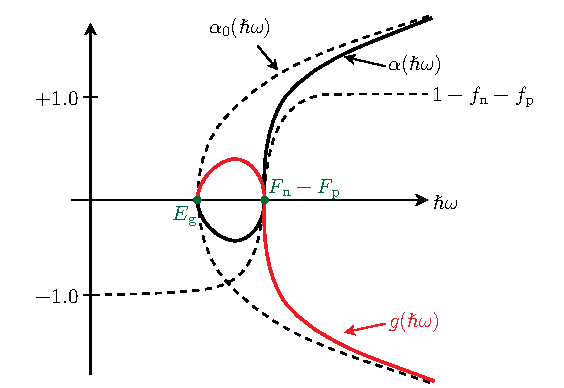
\includegraphics[width=0.6\linewidth]{../assets/absorption_gain.pdf}
	\caption{Absorption coefficient $\alpha(\hbar\omega)$ under carrier injection
	(solid) compared to the equilibrium absorption $\alpha_{0}(\hbar\omega)$ (dashed).
	The factor $1-f_{\mathrm{n}}-f_{\mathrm{p}}$ (dashed) changes sign at $\hbar\omega
	=F_{\mathrm{n}}-F_{\mathrm{p}}$. The gain
	$g(\hbar\omega)=-\alpha(\hbar\omega)$ is shown in red. \imcite{chuang_physics_2009}}
	\label{fig:absorption_gain}
\end{figure}

Note that $g$ is the material gain of the active medium alone. The gain
experienced by a guided optical mode is reduced to the modal gain $\Gamma g$ by
the optical confinement factor $\Gamma$. Lasing additionally requires this modal gain
to overcome the internal losses and the mirror losses (see
\cref{sec:resonator_and_threshold}).

% Gliederung: Brücke zu Kapitel 4: der Fabry-Perot-Resonator braucht $g$ für die Schwellbedingung $\Gamma g_{\mathrm{th}}=\alpha_{\mathrm i}+\alpha_{\mathrm m}$
	% !TEX root = ../main.tex
\section{Laser Diode}
\label{sec:laser_diode}

The earliest semiconductor lasers were homojunction lasers, which were
demonstrated in 1962. These “proof of concept” lasers featured a threshold
current density of $\SI{19000}{A/cm^{2}}$ at cryogenic temperature. A prominent vertical
layer structure that was realized in 1969–1970 is the Double Heterostructure. In
comparison to homojunctions, a double heterostructure (DHS) featured a significantly
lower threshold current density ($\SI{1600}{A/cm^{2}}$) and could be operated at room
temperature.

However, almost all commercial laser diodes today are no longer simple double-heterostructure
lasers but quantum-well lasers, usually with a separate-confinement heterostructure
(SCH). The first single and multiple quantum-well lasers were demonstrated in
1977 by Holonyak’s group using liquid-phase epitaxy. Confining the electron-hole pairs
to the thin well region reduced the threshold current density to about $\SI{500}{A/cm^{2}}$.
Introducing strain into the quantum wells in the late 1980s lowered it further
to $\SI{65}{A/cm^{2}}$ at room temperature.

\subsection{Vertical Structure}
\label{sec:vertical_structure}

A thin layer of low-band-gap material is embedded between two layers of higher-band-gap
material. See \cref{fig:double_heterostructure}. The band-gap step confines
charge carriers and the refractive-index step confines light, both in the same thin
layer. A popular material system is $\ce{GaAs}$ as gain medium with
$\ce{AlGaAs}$ as cladding.

\begin{figure}
	\centering
	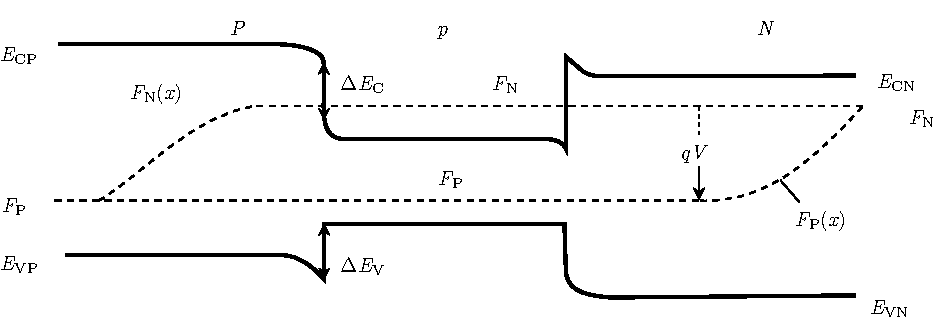
\includegraphics[width=\linewidth]{../assets/band_diagram.pdf}
	\caption{Band diagram of a $P$-$p$-$N$ double heterostructure under forward
	bias $V$. \imcite{chuang_physics_2009}}
	\label{fig:double_heterostructure}
\end{figure}

The band offsets form potential wells that trap injected charge carriers in the low-gap
layer, where they recombine. However, carriers with an energy higher than the
barrier height can pass over the barrier, escape from the well and no longer recombine
in the active layer. This effect results in a leakage current $I_{\mathrm{L}}$.

In the transparent regime, $\epsilon'' \simeq 0$ and $n_{\mathrm{r}}\simeq \sqrt{
\epsilon'}$. Using the oscillator model:
\begin{equation}
	\epsilon'=1 + \int \frac{e^{2}}{\epsilon_{0}m_{0}\omega_{\mathrm{cv}}^{2}}\frac{2
	\lvert \mathbf{p}_{\mathrm{cv}}\rvert^{2}}{m_{0}\hbar \omega_{\mathrm{cv}}}\frac{1}{1-\omega^{2}/\omega_{\mathrm{cv}}^{2}}
	\, \frac{\mathrm{d}\mathbf{k}}{(2\pi)^{3}}
\end{equation}

% \begin{table}[H]
% \centering
% \begin{tabular}{p{0.32\textwidth}p{0.32\textwidth}p{0.32\textwidth}}
% \toprule
% Symbol & Meaning & Unit \\
% \midrule
% $\epsilon'$ & real part of the relative dielectric function & dimensionless \\
% $e$ & elementary charge & $\mathrm{C}$ \\
% $\epsilon_{0}$ & vacuum permittivity & $\mathrm{F\,m^{-1}}$ \\
% $m_{0}$ & free electron mass & $\mathrm{kg}$ \\
% $\omega_{\mathrm{cv}}$ & angular frequency of the interband transition at $\mathbf{k}$, $\hbar\omega_{\mathrm{cv}}=E_{\mathrm{c}}(\mathbf{k})-E_{\mathrm{v}}(\mathbf{k})$ & $\mathrm{rad\,s^{-1}}$ \\
% $\mathbf{p}_{\mathrm{cv}}$ & momentum matrix element between conduction- and valence-band states & $\mathrm{kg\,m\,s^{-1}}$ \\
% $\hbar$ & reduced Planck constant & $\mathrm{J\,s}$ \\
% $\omega$ & angular frequency of the light & $\mathrm{rad\,s^{-1}}$ \\
% $\mathbf{k}$ & wavevector of the electronic states & $\mathrm{m^{-1}}$ \\
% \bottomrule
% \end{tabular}
% \caption{TODO}
% \end{table}

If the band-gap energy decreases, $\omega_{\mathrm{cv}}$ decreases, so that all factors
of the integrand increase. Hence, both $\epsilon'$ and $n_{\mathrm{r}}$ increase.
A low-gap layer consequently has a higher refractive index than its surroundings,
leading to wave guiding in this layer. The layer acts like the core of a glass
fiber in which light is guided (see \cref{fig:refractive_index_profile}).

\begin{figure}[H]
	\centering
	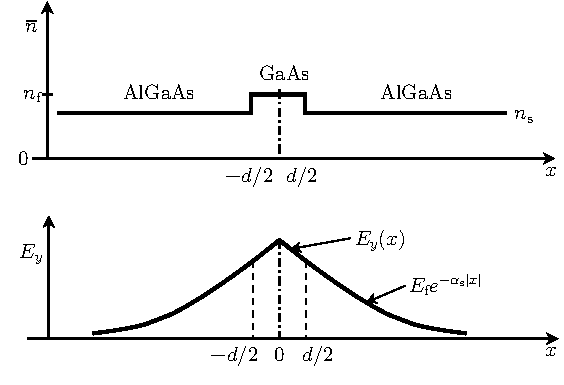
\includegraphics[width=0.6\linewidth]{../assets/refractive_index_profile.pdf}
	\caption{Profile of the refractive index $\bar n$ of an AlGaAs/GaAs double
	heterostructure (top) with the core index $n_{\mathrm{f}}$ and the cladding
	index $n_{\mathrm{s}}$, and approximate field distribution $E_{y}(x)$ of the guided
	optical wave (bottom). The field is approximated by an exponential decay
	$E_{\mathrm{f}}e^{-\alpha_{\mathrm{s}}\lvert x\rvert}$ with the peak amplitude
	$E_{\mathrm{f}}$ and the decay constant $\alpha_{\mathrm{s}}$ in the cladding. \imcite{ebeling_integrated_1993}}
	\label{fig:refractive_index_profile}
\end{figure}

% Gliederung: [[Optical Confinement Factor]]
% ---- Optical Confinement Factor.md ----

A key metric is the Optical Confinement Factor $\Gamma$. It is the fraction of the
light intensity, integrated over the cross section, that lies within a specified region.
For a one-dimensional problem in which the specified region is centered at the
origin and has the width $d$, $\Gamma$ can be expressed as:
\begin{equation}
	\Gamma=\frac{\int_{-d /2}^{d /2}\lvert E(x) \rvert^{2}\, \mathrm{d}x}{\int_{-\infty}^{\infty}\lvert
	E(x) \rvert^{2}\, \mathrm{d}x}
\end{equation}

% \begin{table}[H]
% \centering
% \begin{tabular}{p{0.32\textwidth}p{0.32\textwidth}p{0.32\textwidth}}
% \toprule
% Symbol & Meaning & Unit \\
% \midrule
% $\Gamma$ & optical confinement factor & dimensionless \\
% $E$ & electric field amplitude of the guided mode & $\mathrm{V\,m^{-1}}$ \\
% $x$ & position perpendicular to the layers & $\mathrm{m}$ \\
% $d$ & width of the specified region (e.g. active layer thickness) & $\mathrm{m}$ \\
% \bottomrule
% \end{tabular}
% \caption{TODO}
% \end{table}

The confinement factor of the gain region is used as a figure of merit in laser
diodes. A value of $\Gamma$ close to one is desirable.

\subsection{Lateral Structure}
\label{sec:lateral_structure}

% Gliederung: [[Laser Diode]]: Abschnitte zur Schichtstruktur und lateralen Struktur (Gain Guiding, Index Guiding)
% ---- Laser Diode.md ----

The lateral structure confines current and light in the direction parallel to
the layers; the two common approaches are gain guiding and index guiding (see
\cref{fig:gain_index_guiding}).

To achieve a high current density at low external currents, the current is
injected only into a narrow stripe. For this purpose, the surface contact is
insulated by an oxide layer everywhere except for a narrow stripe running
parallel to the cavity. Since optical gain only occurs where carriers are injected,
the current density profile also determines the lateral extension of the light
wave. This mechanism is known as “gain guiding”.

In a ridge waveguide structure, the p-type layer is etched away except for a
small stripe, the so-called mesa. As a result, the effective thickness of the p-AlGaAs
cladding layer differs between the region below the mesa and its surroundings,
which changes the effective refractive index. Since the effective refractive index
is higher below the mesa, the wave is guided in this region. This mechanism is known
as “index guiding”.

\begin{figure}[H]
	\centering
	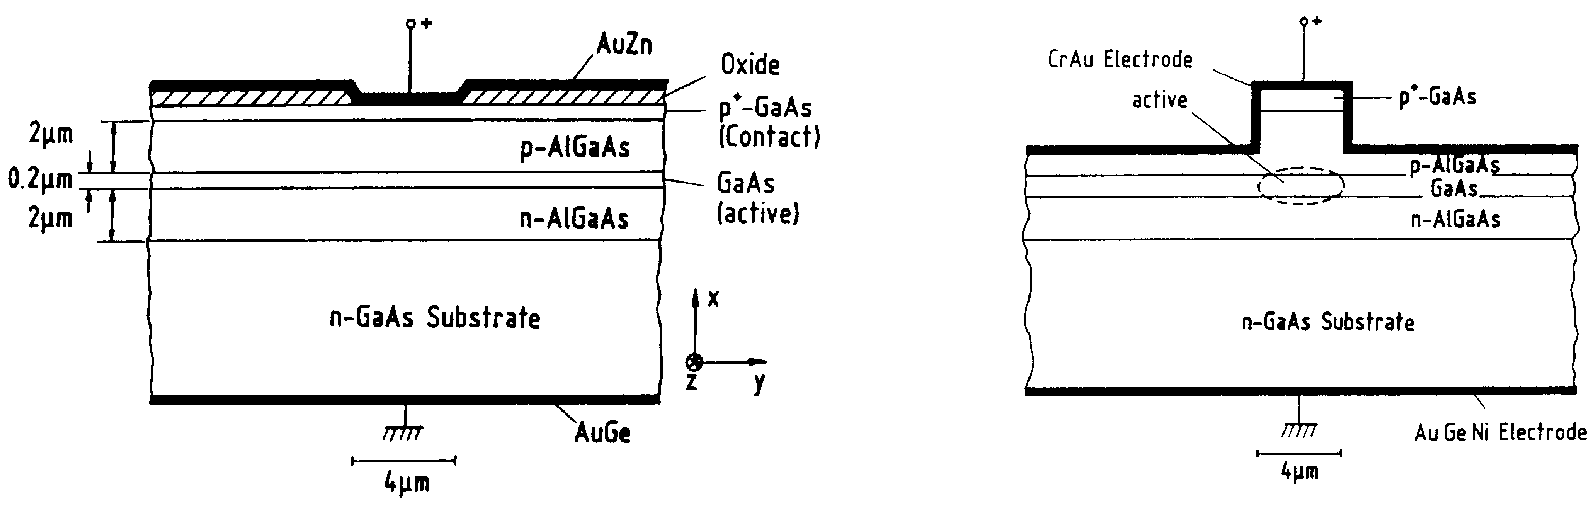
\includegraphics[width=\linewidth]{../assets/gain_index_guiding.png}
	\caption{Cross section of an oxide stripe laser (left) as an example for gain
	guiding and a ridge waveguide laser (right) as an example for index guiding. \imcite{ebeling_integrated_1993}}
	\label{fig:gain_index_guiding}
\end{figure}

\subsection{Resonator and Threshold}
\label{sec:resonator_and_threshold}

% Gliederung: [[Fabry-Perot Resonator]]
% ---- Fabry-Perot Resonator.md ----

A crucial part of a laser is a resonator that feeds part of the light back into the
amplifying medium. This resonator consists of two plane-parallel mirrors. In semiconductor
lasers, the mirrors are realized as smooth cleaved facets at both ends of the
active stripe. A laser oscillates when a light wave returns after one round trip with
identical amplitude and phase. The gain must then exactly compensate all losses.

The cleaved facets act as mirrors through Fresnel reflection at the
semiconductor–air interface; at normal incidence, the reflectivity is:
\begin{equation}
	R=\left(\frac{\bar n-1}{\bar n+1}\right)^{2}
\end{equation}

% \begin{table}[H]
% \centering
% \begin{tabular}{p{0.32\textwidth}p{0.32\textwidth}p{0.32\textwidth}}
% \toprule
% Symbol & Meaning & Unit \\
% \midrule
% $R$ & intensity reflectivity of a cleaved facet & dimensionless \\
% $\bar n$ & effective refractive index of the mode & dimensionless \\
% \bottomrule
% \end{tabular}
% \caption{TODO}
% \end{table}

\subsubsection{Round-Trip Condition}

The light intensity of the guided mode grows with the modal gain $\Gamma g$ and
decays with the intrinsic loss $\alpha_{\mathrm{i}}$. As the electric field amplitude
scales with the square root of the intensity, it varies along the cavity as:
\begin{equation}
	E(z)=E_{0}\exp\left[\tfrac{1}{2}(\Gamma g-\alpha_{\mathrm{i}})z\right]\exp(\mathrm{i}
	\beta z),\qquad \beta=\frac{2\pi\bar n}{\lambda}
\end{equation}

% \begin{table}[H]
% \centering
% \begin{tabular}{p{0.32\textwidth}p{0.32\textwidth}p{0.32\textwidth}}
% \toprule
% Symbol & Meaning & Unit \\
% \midrule
% $E(z), E_0$ & electric field amplitude of the mode along the cavity / at $z=0$ & $\mathrm{V\,m^{-1}}$ \\
% $z$ & position along the cavity axis & $\mathrm{m}$ \\
% $\Gamma$ & optical confinement factor & dimensionless \\
% $g$ & material gain coefficient & $\mathrm{m^{-1}}$ \\
% $\alpha_{\mathrm i}$ & intrinsic loss & $\mathrm{m^{-1}}$ \\
% $\beta$ & propagation constant of the mode & $\mathrm{m^{-1}}$ \\
% $\bar n$ & effective refractive index of the mode & dimensionless \\
% $\lambda$ & vacuum wavelength & $\mathrm{m}$ \\
% \bottomrule
% \end{tabular}
% \caption{TODO}
% \end{table}

The intrinsic loss $\alpha_{\mathrm{i}}$ originates from free-carrier absorption in
the waveguide materials and from scattering at rough waveguide walls. At each
facet only the fraction $r_{1}$ or $r_{2}$ of the field amplitude is reflected. After
a round trip (length $2L$, two reflections) the field has to reproduce itself:
\begin{equation}
	r_{1} r_{2}\,\exp\left[(\Gamma g-\alpha_{\mathrm{i}})L\right]\exp(2\mathrm{i}\beta
	L)=1
\end{equation}

% \begin{table}[H]
% \centering
% \begin{tabular}{p{0.32\textwidth}p{0.32\textwidth}p{0.32\textwidth}}
% \toprule
% Symbol & Meaning & Unit \\
% \midrule
% $r_1, r_2$ & amplitude reflection coefficients of the two facets, $R_{1,2}=\lvert r_{1,2}\rvert^2$ & dimensionless \\
% $\Gamma$ & optical confinement factor & dimensionless \\
% $g$ & material gain coefficient & $\mathrm{m^{-1}}$ \\
% $\alpha_{\mathrm i}$ & intrinsic loss & $\mathrm{m^{-1}}$ \\
% $L$ & length of the laser cavity & $\mathrm{m}$ \\
% $\beta$ & propagation constant of the mode & $\mathrm{m^{-1}}$ \\
% \bottomrule
% \end{tabular}
% \caption{TODO}
% \end{table}

As this condition is complex-valued, it splits into one condition for the
magnitude (threshold) and one for the phase (modes).

\paragraph{Amplitude Condition: Threshold}

Since the reflectivities $R_{1/2}$ refer to intensities, the amplitude reflection
coefficients are their square roots, $r_{1}r_{2}=\sqrt{R_{1}R_{2}}$. The magnitude
of the round-trip condition fixes the gain needed at threshold:
\begin{equation}
	\sqrt{R_{1}R_{2}}\,\exp\left[(\Gamma g_{\mathrm{th}}-\alpha_{\mathrm{i}})L\right
	]\overset{!}{=}1 \quad\Rightarrow\quad \Gamma g_{\mathrm{th}}=\alpha_{\mathrm{i}}
	+\underbrace{\frac{1}{2L}\ln\frac{1}{R_{1}R_{2}}}_{\alpha_{\mathrm{m}}}=\alpha_{\mathrm{i}}
	+\alpha_{\mathrm{m}}
\end{equation}
% \begin{table}[H]
% \centering
% \begin{tabular}{p{0.32\textwidth}p{0.32\textwidth}p{0.32\textwidth}}
% \toprule
% Symbol & Meaning & Unit \\
% \midrule
% $R_1, R_2$ & intensity reflectivities of the two facets & dimensionless \\
% $\Gamma$ & optical confinement factor & dimensionless \\
% $g_{\mathrm{th}}$ & gain coefficient at threshold & $\mathrm{m^{-1}}$ \\
% $\alpha_{\mathrm i}$ & intrinsic loss & $\mathrm{m^{-1}}$ \\
% $\alpha_{\mathrm m}$ & mirror loss & $\mathrm{m^{-1}}$ \\
% $L$ & length of the laser cavity & $\mathrm{m}$ \\
% \bottomrule
% \end{tabular}
% \caption{TODO}
% \end{table}
The mirror loss $\alpha_{\mathrm{m}}$ accounts for the light leaving through the
facets, which forms the useful laser output. At threshold, the modal gain balances
the intrinsic and mirror losses.

\paragraph{Phase Condition: Longitudinal Modes}

The phase of the round-trip condition has to be a multiple of $2\pi$:
\begin{equation}
	2\beta L\overset{!}{=}2\pi m\quad\Rightarrow\quad m\lambda=2L\bar n
\end{equation}
% \begin{table}[H]
% \centering
% \begin{tabular}{lll}
% \toprule
% Symbol & Meaning & Unit \\
% \midrule
% $m$ & longitudinal mode number & dimensionless (integer) \\
% $\beta$ & propagation constant of the mode & $\mathrm{m^{-1}}$ \\
% $L$ & length of the laser cavity & $\mathrm{m}$ \\
% $\lambda$ & vacuum wavelength & $\mathrm{m}$ \\
% $\bar n$ & effective refractive index of the mode & dimensionless \\
% \bottomrule
% \end{tabular}
% \caption{TODO}
% \end{table}
The amplitude condition decides whether a mode lases, and the phase condition at which
wavelength it lases. Using finite difference approximation as
$\Delta m /\Delta\lambda \simeq \partial_{\lambda}m$, the mode separation for large
$m$ is given as:
\begin{equation}
	\Delta\lambda=\frac{\lambda^{2}\Delta m}{2\bar{n}L[1-(\lambda /\bar{n})(\mathrm{d}\bar{n}/\mathrm{d}\lambda)]}
\end{equation}

% \begin{table}[H]
% \centering
% \begin{tabular}{p{0.32\textwidth}p{0.32\textwidth}p{0.32\textwidth}}
% \toprule
% Symbol & Meaning & Unit \\
% \midrule
% $\Delta\lambda$ & wavelength spacing between modes & $\mathrm{m}$ \\
% $\Delta m$ & difference in mode number & dimensionless (integer) \\
% $\lambda$ & vacuum wavelength & $\mathrm{m}$ \\
% $\bar n$ & effective refractive index of the mode & dimensionless \\
% $\mathrm{d}\bar n/\mathrm{d}\lambda$ & dispersion of the effective refractive index & $\mathrm{m^{-1}}$ \\
% $L$ & length of the laser cavity & $\mathrm{m}$ \\
% \bottomrule
% \end{tabular}
% \caption{TODO}
% \end{table}

\subsection{P-I Characteristic}
\label{sec:p_i_characteristic}

% Gliederung: [[Laser Diode P-I Curve]]: verwendet $\Gamma$, $\alpha_{\mathrm m}$, $g_{\mathrm{th}}$ und $I_{\mathrm L}$ aus den vorherigen Abschnitten
% ---- Laser Diode P-I Curve.md ----

A rate equation can be used to
describe the dynamics of the carrier density $n$ and the Photon Density $S$:
\begin{equation}
	\frac{\mathrm{d}n(t)}{\mathrm{d}t}= \eta_{\mathrm{i}}\frac{j(t)}{qd}- R(n) - v_{\mathrm{g}}
	g(n) S(t)
\end{equation}

% \begin{table}[H]
% \centering
% \begin{tabular}{lll}
% \toprule
% Symbol & Meaning & Unit \\
% \midrule
% $n$ & carrier density & $\mathrm{m^{-3}}$ \\
% $t$ & time & $\mathrm{s}$ \\
% $\eta_{\mathrm i}$ & collection efficiency & dimensionless \\
% $j$ & injection current density & $\mathrm{A\,m^{-2}}$ \\
% $q$ & elementary charge & $\mathrm{C}$ \\
% $d$ & thickness of the active region & $\mathrm{m}$ \\
% $R(n)$ & recombination rate per volume & $\mathrm{m^{-3}\,s^{-1}}$ \\
% $v_{\mathrm g}$ & group velocity of the light & $\mathrm{m\,s^{-1}}$ \\
% $g(n)$ & material gain coefficient & $\mathrm{m^{-1}}$ \\
% $S$ & photon density & $\mathrm{m^{-3}}$ \\
% \bottomrule
% \end{tabular}
% \caption{TODO}
% \end{table}

The first term on the right hand side describes the carrier injection into the active region with
thickness $d$ and collection efficiency $\eta_{\mathrm{i}}$. $R(n)$ represents (radiative
and nonradiative) recombination processes. The last term expresses the carrier
loss due to stimulated emission.

Using the ABC model, the recombination rate is given as:
\begin{align}
	R(n)    & =An +Bn^{2}+Cn^{3}=\frac{n}{\tau(n)} \\
	\tau(n) & =(A+Bn+Cn^{2})^{-1}
\end{align}
% \begin{table}[H]
% \centering
% \begin{tabular}{p{0.32\textwidth}p{0.32\textwidth}p{0.32\textwidth}}
% \toprule
% Symbol & Meaning & Unit \\
% \midrule
% $R(n)$ & recombination rate per volume & $\mathrm{m^{-3}\,s^{-1}}$ \\
% $\tau(n)$ & carrier lifetime & $\mathrm{s}$ \\
% $n$ & carrier density & $\mathrm{m^{-3}}$ \\
% $A, B, C$ & coefficients for defect, radiative and Auger recombination & $\mathrm{s^{-1}}$, $\mathrm{m^{3}\,s^{-1}}$, $\mathrm{m^{6}\,s^{-1}}$ \\
% \bottomrule
% \end{tabular}
% \caption{TODO}
% \end{table}
where $An$ represents nonradiative recombination of carriers with defects, $Bn^{2}$
the spontaneous emission and $Cn^{3}$ the nonradiative Auger recombination.

\paragraph{Steady State with Low Current Density}

In steady state and at low current density, the carrier concentration is determined
by the injection current. As the photon density is negligible ($S \simeq 0$), it follows
that:
\begin{equation}
	\eta_{\mathrm{i}}\frac{j}{qd}=\frac{n}{\tau}
\end{equation}

% \begin{table}[H]
% \centering
% \begin{tabular}{lll}
% \toprule
% Symbol & Meaning & Unit \\
% \midrule
% $\eta_{\mathrm i}$ & collection efficiency & dimensionless \\
% $j$ & injection current density & $\mathrm{A\,m^{-2}}$ \\
% $q$ & elementary charge & $\mathrm{C}$ \\
% $d$ & thickness of the active region & $\mathrm{m}$ \\
% $n$ & carrier density & $\mathrm{m^{-3}}$ \\
% $\tau$ & carrier lifetime & $\mathrm{s}$ \\
% \bottomrule
% \end{tabular}
% \caption{TODO}
% \end{table}

The carrier density $n$ can be obtained by assuming either a constant $\tau$ or
constant $A, B, C$ parameters. Typically, a linear relation for the peak gain
coefficient versus carrier density is assumed using the differential gain $g'$
and the transparency concentration $n_{\mathrm{tr}}$:
\begin{equation}
	g(n)=g' (n-n_{\mathrm{tr}})
\end{equation}

% \begin{table}[H]
% \centering
% \begin{tabular}{lll}
% \toprule
% Symbol & Meaning & Unit \\
% \midrule
% $g(n)$ & peak material gain coefficient & $\mathrm{m^{-1}}$ \\
% $g'$ & differential gain & $\mathrm{m^{2}}$ \\
% $n$ & carrier density & $\mathrm{m^{-3}}$ \\
% $n_{\mathrm{tr}}$ & transparency carrier density & $\mathrm{m^{-3}}$ \\
% \bottomrule
% \end{tabular}
% \caption{TODO}
% \end{table}

\paragraph{Threshold Condition}

The round-trip condition that is enforced in a Fabry-Perot Resonator (see \cref{sec:resonator_and_threshold}) results in
a threshold condition of the material gain:
\begin{equation}
	\Gamma g_{\mathrm{th}}=\alpha_{\mathrm{i}}+\alpha_{\mathrm{m}}
\end{equation}

% \begin{table}[H]
% \centering
% \begin{tabular}{lll}
% \toprule
% Symbol & Meaning & Unit \\
% \midrule
% $\Gamma$ & optical confinement factor & dimensionless \\
% $g_{\mathrm{th}}$ & gain coefficient at threshold & $\mathrm{m^{-1}}$ \\
% $\alpha_{\mathrm i}$ & intrinsic loss & $\mathrm{m^{-1}}$ \\
% $\alpha_{\mathrm m}$ & mirror loss & $\mathrm{m^{-1}}$ \\
% \bottomrule
% \end{tabular}
% \caption{TODO}
% \end{table}

The modal gain $\Gamma
g_{\mathrm{th}}$ must equal the sum of the intrinsic loss $\alpha_{\mathrm{i}}$ and
the mirror loss $\alpha_{\mathrm{m}}$. With increasing $j$, $n$ increases and therefore
$g$ increases up to its threshold value. Consequently, $g_{\mathrm{th}}$ limits $n$
to $n_{\mathrm{th}}$, which is reached for $j=j_{\mathrm{th}}$.
\begin{align}
	g_{\mathrm{th}} & =\frac{\alpha_{\mathrm{i}}+\alpha_{\mathrm{m}}}{\Gamma}                                   \\
	n_{\mathrm{th}} & =n_{\mathrm{tr}}+(\alpha_{\mathrm{i}}+\alpha_{\mathrm{m}}) /(\Gamma g')                   \\
	j_{\mathrm{th}} & =\frac{qd}{\eta_{\mathrm{i}}}(An_{\mathrm{th}}+Bn_{\mathrm{th}}^{2}+Cn_{\mathrm{th}}^{3}) \label{eq:j_th}
\end{align}

% \begin{table}[H]
% \centering
% \begin{tabular}{p{0.32\textwidth}p{0.32\textwidth}p{0.32\textwidth}}
% \toprule
% Symbol & Meaning & Unit \\
% \midrule
% $g_{\mathrm{th}}$ & gain coefficient at threshold & $\mathrm{m^{-1}}$ \\
% $\alpha_{\mathrm i}$ & intrinsic loss & $\mathrm{m^{-1}}$ \\
% $\alpha_{\mathrm m}$ & mirror loss & $\mathrm{m^{-1}}$ \\
% $\Gamma$ & optical confinement factor & dimensionless \\
% $n_{\mathrm{th}}$ & carrier density at threshold & $\mathrm{m^{-3}}$ \\
% $n_{\mathrm{tr}}$ & transparency carrier density & $\mathrm{m^{-3}}$ \\
% $g'$ & differential gain & $\mathrm{m^{2}}$ \\
% $j_{\mathrm{th}}$ & threshold current density & $\mathrm{A\,m^{-2}}$ \\
% $q$ & elementary charge & $\mathrm{C}$ \\
% $d$ & thickness of the active region & $\mathrm{m}$ \\
% $\eta_{\mathrm i}$ & collection efficiency & dimensionless \\
% $A, B, C$ & coefficients for defect, radiative and Auger recombination & $\mathrm{s^{-1}}$, $\mathrm{m^{3}\,s^{-1}}$, $\mathrm{m^{6}\,s^{-1}}$ \\
% \bottomrule
% \end{tabular}
% \caption{TODO}
% \end{table}

\paragraph{Light Power Output}

The laser diode output consists of spontaneous emission below the threshold
current density. A further increase of $j$ above threshold increases the photon density
$S$ directly:
\begin{equation}
	\eta_{\mathrm{i}}\frac{j}{qd}= (An_{\mathrm{th}}+Bn^{2}_{\mathrm{th}}+C n^{3}_{\mathrm{th}}
	) +v_{\mathrm{g}}g_{\mathrm{th}}S \quad \text{ for }j>j_{\mathrm{th}}
\end{equation}

% \begin{table}[H]
% \centering
% \begin{tabular}{p{0.32\textwidth}p{0.32\textwidth}p{0.32\textwidth}}
% \toprule
% Symbol & Meaning & Unit \\
% \midrule
% $\eta_{\mathrm i}$ & collection efficiency & dimensionless \\
% $j$ & injection current density & $\mathrm{A\,m^{-2}}$ \\
% $q$ & elementary charge & $\mathrm{C}$ \\
% $d$ & thickness of the active region & $\mathrm{m}$ \\
% $A, B, C$ & coefficients for defect, radiative and Auger recombination & $\mathrm{s^{-1}}$, $\mathrm{m^{3}\,s^{-1}}$, $\mathrm{m^{6}\,s^{-1}}$ \\
% $n_{\mathrm{th}}$ & carrier density at threshold & $\mathrm{m^{-3}}$ \\
% $v_{\mathrm g}$ & group velocity of the light & $\mathrm{m\,s^{-1}}$ \\
% $g_{\mathrm{th}}$ & gain coefficient at threshold & $\mathrm{m^{-1}}$ \\
% $S$ & photon density & $\mathrm{m^{-3}}$ \\
% \bottomrule
% \end{tabular}
% \caption{TODO}
% \end{table}

Subtracting \cref{eq:j_th} results in a simple linear
relationship between photon density and injection current density above
threshold:
\begin{equation}
	S=\eta_{\mathrm{i}}\frac{j-j_{\mathrm{th}}}{qd v_{\mathrm{g}}g_{\mathrm{th}}}
	\label{eq:photon_density}
\end{equation}

% \begin{table}[H]
% \centering
% \begin{tabular}{lll}
% \toprule
% Symbol & Meaning & Unit \\
% \midrule
% $S$ & photon density & $\mathrm{m^{-3}}$ \\
% $\eta_{\mathrm i}$ & collection efficiency & dimensionless \\
% $j, j_{\mathrm{th}}$ & injection / threshold current density & $\mathrm{A\,m^{-2}}$ \\
% $q$ & elementary charge & $\mathrm{C}$ \\
% $d$ & thickness of the active region & $\mathrm{m}$ \\
% $v_{\mathrm g}$ & group velocity of the light & $\mathrm{m\,s^{-1}}$ \\
% $g_{\mathrm{th}}$ & gain coefficient at threshold & $\mathrm{m^{-1}}$ \\
% \bottomrule
% \end{tabular}
% \caption{TODO}
% \end{table}

The output power $P_{\mathrm{out}}$ is the (energy of a photon) times the (number of
photons in the optical mode) times the (rate at which photons escape through the mirrors):
\begin{equation}
	P_{\mathrm{out}}=\hbar\omega\, S\,(wLd_{\mathrm{op}})\,(v_{\mathrm{g}}\alpha_{\mathrm{m}}
	)
\end{equation}

% \begin{table}[H]
% \centering
% \begin{tabular}{p{0.32\textwidth}p{0.32\textwidth}p{0.32\textwidth}}
% \toprule
% Symbol & Meaning & Unit \\
% \midrule
% $P_{\mathrm{out}}$ & optical output power through both mirrors & $\mathrm{W}$ \\
% $\hbar\omega$ & photon energy & $\mathrm{J}$ (often eV) \\
% $S$ & photon density & $\mathrm{m^{-3}}$ \\
% $w$ & width of the optical mode & $\mathrm{m}$ \\
% $L$ & length of the laser cavity & $\mathrm{m}$ \\
% $d_{\mathrm{op}}$ & effective thickness of the optical mode & $\mathrm{m}$ \\
% $v_{\mathrm g}$ & group velocity of the light & $\mathrm{m\,s^{-1}}$ \\
% $\alpha_{\mathrm m}$ & mirror loss & $\mathrm{m^{-1}}$ \\
% \bottomrule
% \end{tabular}
% \caption{TODO}
% \end{table}

In this equation, $wLd_{\mathrm{op}}$ is the effective volume of the optical mode,
so $S\,(wLd_{\mathrm{op}})$ is the number of photons in the mode, and $v_{\mathrm{g}}
\alpha_{\mathrm{m}}$ is the escape rate per photon. Substituting $S$ from \cref{eq:photon_density}, using $I=jw
L$, $I_{\mathrm{th}}=j_{\mathrm{th}}wL$, $g_{\mathrm{th}}=(\alpha_{\mathrm{i}}+\alpha
_{\mathrm{m}})/\Gamma$ and the confinement factor $\Gamma=d/d_{\mathrm{op}}$ (ratio
of active-region thickness to optical-mode thickness), yields the well-known
$P_{\mathrm{out}}(I)$ curve:
\begin{equation}
	P_{\mathrm{out}}=\underbrace{ \eta_{\mathrm{i}} \frac{\alpha_{\mathrm{m}}}{\alpha_{\mathrm{i}}+\alpha_{\mathrm{m}}}
	}_{ \eta_{\mathrm{d}} }\frac{\hbar \omega}{q}(I-I_{\mathrm{th}})
\end{equation}

% \begin{table}[H]
% \centering
% \begin{tabular}{lll}
% \toprule
% Symbol & Meaning & Unit \\
% \midrule
% $P_{\mathrm{out}}$ & optical output power & $\mathrm{W}$ \\
% $\eta_{\mathrm i}$ & collection efficiency & dimensionless \\
% $\alpha_{\mathrm m}$ & mirror loss & $\mathrm{m^{-1}}$ \\
% $\alpha_{\mathrm i}$ & intrinsic loss & $\mathrm{m^{-1}}$ \\
% $\eta_{\mathrm d}$ & external differential quantum efficiency & dimensionless \\
% $\hbar\omega$ & photon energy & $\mathrm{J}$ (often eV) \\
% $q$ & elementary charge & $\mathrm{C}$ \\
% $I$ & injection current & $\mathrm{A}$ \\
% $I_{\mathrm{th}}$ & threshold current & $\mathrm{A}$ \\
% \bottomrule
% \end{tabular}
% \caption{TODO}
% \end{table}

The slope of the normalized curve $P_{\mathrm{out}}/(\hbar \omega)$ versus $I /q$
is the external differential quantum efficiency $\eta_{\mathrm{d}}$. In contrast,
the wall-plug efficiency is defined as $P_{\mathrm{out}}/ (VI)$ with the applied voltage
$V$.

\paragraph{Real Devices}

In real devices, a leakage current exists due to the finite barrier height in the
double heterostructure. The model can be extended by splitting the total current
into the current injected into the active region $I_{\mathrm{A}}$ and the
leakage current $I_{\mathrm{L}}$. If $I_{\mathrm{th}}$ additionally includes the threshold
leakage current, $P_{\mathrm{out}}$ can be described as
\begin{equation}
	P_{\mathrm{out}}=\eta_{\mathrm{i}}\frac{\hbar \omega}{q}\frac{\alpha_{\mathrm{m}}}{\alpha_{\mathrm{m}}+\alpha_{\mathrm{i}}}
	(I-I_{\mathrm{th}}-\Delta I_{\mathrm{L}})
\end{equation}

% \begin{table}[H]
% \centering
% \begin{tabular}{p{0.32\textwidth}p{0.32\textwidth}p{0.32\textwidth}}
% \toprule
% Symbol & Meaning & Unit \\
% \midrule
% $P_{\mathrm{out}}$ & optical output power & $\mathrm{W}$ \\
% $\eta_{\mathrm i}$ & collection efficiency & dimensionless \\
% $\hbar\omega$ & photon energy & $\mathrm{J}$ (often eV) \\
% $q$ & elementary charge & $\mathrm{C}$ \\
% $\alpha_{\mathrm m}$ & mirror loss & $\mathrm{m^{-1}}$ \\
% $\alpha_{\mathrm i}$ & intrinsic loss & $\mathrm{m^{-1}}$ \\
% $I$ & injection current & $\mathrm{A}$ \\
% $I_{\mathrm{th}}$ & threshold current (including the threshold leakage current) & $\mathrm{A}$ \\
% $\Delta I_{\mathrm L}$ & additional leakage current caused by the increase of $I$ above $I_{\mathrm{th}}$ & $\mathrm{A}$ \\
% \bottomrule
% \end{tabular}
% \caption{TODO}
% \end{table}

Up to the threshold current, only a slight increase in optical power is measured.
In this regime, the diode effectively operates as an LED. For currents above the
threshold current, the (steep) linear relationship is established, as discussed
above. For high currents, the output power saturates. Possible causes are:

\begin{itemize}
	\item An increased leakage current $\Delta I_{\mathrm{L}}(I)$

	\item A current dependence of the threshold current due to junction heating

	\item A current dependence of the intrinsic loss $\alpha_{\mathrm{i}}$
\end{itemize}

The threshold current density is often expressed as a function of temperature,
using an empirical formula with the characteristic temperature $T_{0}$ over a
temperature range near $T_{1}$:
\begin{equation}
	j_{\mathrm{th}}(T)=j_{\mathrm{th}}(T_{1}) \exp\left(\frac{T-T_{1}}{T_{0}}\right
	)
\end{equation}

% \begin{table}[H]
% \centering
% \begin{tabular}{lll}
% \toprule
% Symbol & Meaning & Unit \\
% \midrule
% $j_{\mathrm{th}}$ & threshold current density & $\mathrm{A\,m^{-2}}$ \\
% $T$ & temperature & $\mathrm{K}$ \\
% $T_{1}$ & reference temperature & $\mathrm{K}$ \\
% $T_{0}$ & characteristic temperature & $\mathrm{K}$ \\
% \bottomrule
% \end{tabular}
% \caption{TODO}
% \end{table}

A large characteristic temperature is desirable as the threshold current should not
change significantly with temperature. Knowing the geometry of the active region,
the threshold current density can be calculated from the threshold current as $j_{\mathrm{th}}
=I_{\mathrm{th}}/(wL)$.

\begin{figure}[H]
	\centering
	\fbox{\parbox[c][4cm][c]{0.6\textwidth}{\centering
	Platzhalter:\\ \detokenize{Pasted image 20260707221008.png}}}
	\caption{TODO}
\end{figure}

\begin{itemize}
	\item At low operating currents, the spectrum is that of spontaneous emission

	\item With increasing current, the effects of stimulated emission become
		visible

	\item The lines become narrower

	\item Side modes are suppressed at higher currents

	\item At high currents, the laser reaches single-mode operation
\end{itemize}

	\clearpage
	% !TEX root = ../main.tex
% !TEX root = ../main.tex
% Measurement setups (I-U, P-I, spectral), redrawn in TikZ.
% Include with % !TEX root = ../main.tex
% Measurement setups (I-U, P-I, spectral), redrawn in TikZ.
% Include with \input{chapters/measurement_setup.tex}; reference the whole figure
% with \cref{fig:setup} or a single setup with \cref{fig:setup_iu},
% \cref{fig:setup_pi} and \cref{fig:setup_spectral}.

\tikzset{
	setup/.style={font=\small, line width=0.6pt},
	meter/.style={circle, draw, fill=white, minimum size=0.75cm, inner sep=0pt},
	% instrument box with display; terminals (-a) left and (-b) right, origin at (-b)
	instrument/.pic={
		\draw (-2.8,-0.35) rectangle (0.25,1.0);
		\node[draw, rounded corners=2pt, anchor=north west, minimum width=1.2cm,
			minimum height=0.4cm, inner sep=2pt] at (-2.65,0.85) {#1};
		\fill (-0.25,0) circle (2pt) coordinate (-a);
		\fill (0,0) circle (2pt) coordinate (-b);
	},
	ground/.pic={
		\draw (0,0) -- (0,-0.9);
		\draw[line width=1.4pt] (-0.3,-0.9) -- (0.3,-0.9);
	},
	% laser diode pointing to the right, centred at the origin
	diode/.pic={
		\fill (-0.18,0.2) -- (-0.18,-0.2) -- (0.18,0) -- cycle;
		\draw[line width=1.2pt] (0.18,0.2) -- (0.18,-0.2);
	},
	emission/.pic={
		\draw[-{Stealth[length=4pt]}] (-0.15,0.3) -- (0.2,0.7);
		\draw[-{Stealth[length=4pt]}] (0.05,0.3) -- (0.4,0.7);
	},
	% temperature-controlled mount below the diode
	mount/.pic={
		\draw[fill=gray!30] (-0.12,-0.25) rectangle (0.12,-1.0);
		\draw[fill=gray!60] (-0.3,-1.0) rectangle (0.3,-1.15);
	},
}

\begin{figure}[H]
	\centering
	\begin{subfigure}{\linewidth}
		\centering
		\begin{tikzpicture}[setup]
			\path (-3,0) -- (11,0);
			\pic (src) at (0,0) {instrument={$U\!=$}};
			\node[anchor=north west, align=left] at (-2.75,-0.4) {DC voltage\\source};
			\pic at (src-a) {ground};
			\draw (src-b) -- (6.5,0);
			\pic at (3.5,0) {diode};
			\node[above] at (3.5,0.25) {Laser diode};
			\node[meter] at (5.5,0) {A};
			\node[above] at (5.5,0.4) {Ammeter};
			\pic at (6.5,0) {ground};
		\end{tikzpicture}
		\caption{Current-voltage characteristic.}
		\label{fig:setup_iu}
	\end{subfigure}

	\vspace{0.6cm}
	\begin{subfigure}{\linewidth}
		\centering
		\begin{tikzpicture}[setup]
			\path (-3,0) -- (11,0);
			\pic (gen) at (0,0) {instrument={$I\!=$}};
			\node[anchor=north west, align=left] at (-2.75,-0.4) {Pulse\\generator};
			\pic at (gen-a) {ground};
			\draw (gen-b) -- (5.9,0);
			\draw (0.6,0.15) -- (0.9,0.15) -- (0.9,0.6) -- (1.2,0.6) -- (1.2,0.15) -- (1.5,0.15);
			% voltage measurement at the diode
			\fill (2.2,0) circle (2pt);
			\node[meter] (V) at (2.2,-1.0) {U};
			\draw (2.2,0) -- (V);
			\pic at (V.south) {ground};
			% laser diode on mount with detector
			\pic at (3.6,0) {mount};
			\pic at (3.6,0) {diode};
			\pic at (3.6,0) {emission};
			\draw (4.3,0.8) rectangle (5.5,1.1);
			\node[above] at (4.9,1.1) {Detector};
			\node[meter] at (5.1,0) {A};
			\pic at (5.9,0) {ground};
			% lock-in amplifier
			\pic (lock) at (10.5,0) {instrument={Lock-in}};
			\draw (5.5,0.95) -- (6.8,0.95) -- (6.8,-0.6) -- (10.25,-0.6) -- (lock-a);
			\pic at (lock-b) {ground};
		\end{tikzpicture}
		\caption{Optical power-current characteristic.}
		\label{fig:setup_pi}
	\end{subfigure}

	\vspace{0.6cm}
	\begin{subfigure}{\linewidth}
		\centering
		\begin{tikzpicture}[setup]
			\path (-3,0) -- (11,0);
			\pic (src) at (0,0) {instrument={$I\!=$}};
			\node[anchor=north west, align=left] at (-2.75,-0.4) {DC current\\source};
			\pic at (src-a) {ground};
			\draw (src-b) -- (5.3,0);
			\pic at (3.2,0) {mount};
			\pic at (3.2,0) {diode};
			\pic at (3.2,0) {emission};
			\node[meter] at (4.5,0) {A};
			\pic at (5.3,0) {ground};
			% lens focusing onto the monochromator entrance slit
			\draw (4.0,1.25) ellipse (0.12 and 0.42);
			\draw (4.1,1.6) -- (6.0,1.25) -- (4.1,0.9);
			\draw (6.0,0.6) rectangle (9.2,1.9);
			\node[anchor=south east] at (9.2,0.6) {Monochromator};
			\draw (9.2,1.3) rectangle (10.3,1.9);
			\node at (9.75,1.6) {PMT};
			% computer
			\draw[rounded corners=2pt] (7.9,-1.05) rectangle (9.1,0.05);
			\draw[rounded corners=1pt] (8.05,-0.9) rectangle (8.95,-0.1);
			\draw (8.3,-1.05) -- (8.2,-1.3) -- (8.8,-1.3) -- (8.7,-1.05);
			\draw (7.6,-1.3) rectangle (9.6,-1.85);
			\foreach \x in {7.75,7.85,...,8.45} \draw (\x,-1.42) -- (\x,-1.73);
			\draw (8.9,-1.5) rectangle (9.4,-1.65);
			\draw (9.75,1.3) .. controls (9.9,0.0) and (10.1,-1.4) .. (9.6,-1.55);
		\end{tikzpicture}
		\caption{Spectral measurements.}
		\label{fig:setup_spectral}
	\end{subfigure}
	\caption{Measurement setups for the characterisation of the laser diode. The diode
	is placed on a temperature-controlled mount for the P-I and spectral measurements.
	PMT: photomultiplier tube.}
	\label{fig:setup}
\end{figure}
; reference the whole figure
% with \cref{fig:setup} or a single setup with \cref{fig:setup_iu},
% \cref{fig:setup_pi} and \cref{fig:setup_spectral}.

\tikzset{
	setup/.style={font=\small, line width=0.6pt},
	meter/.style={circle, draw, fill=white, minimum size=0.75cm, inner sep=0pt},
	% instrument box with display; terminals (-a) left and (-b) right, origin at (-b)
	instrument/.pic={
		\draw (-2.8,-0.35) rectangle (0.25,1.0);
		\node[draw, rounded corners=2pt, anchor=north west, minimum width=1.2cm,
			minimum height=0.4cm, inner sep=2pt] at (-2.65,0.85) {#1};
		\fill (-0.25,0) circle (2pt) coordinate (-a);
		\fill (0,0) circle (2pt) coordinate (-b);
	},
	ground/.pic={
		\draw (0,0) -- (0,-0.9);
		\draw[line width=1.4pt] (-0.3,-0.9) -- (0.3,-0.9);
	},
	% laser diode pointing to the right, centred at the origin
	diode/.pic={
		\fill (-0.18,0.2) -- (-0.18,-0.2) -- (0.18,0) -- cycle;
		\draw[line width=1.2pt] (0.18,0.2) -- (0.18,-0.2);
	},
	emission/.pic={
		\draw[-{Stealth[length=4pt]}] (-0.15,0.3) -- (0.2,0.7);
		\draw[-{Stealth[length=4pt]}] (0.05,0.3) -- (0.4,0.7);
	},
	% temperature-controlled mount below the diode
	mount/.pic={
		\draw[fill=gray!30] (-0.12,-0.25) rectangle (0.12,-1.0);
		\draw[fill=gray!60] (-0.3,-1.0) rectangle (0.3,-1.15);
	},
}

\begin{figure}[H]
	\centering
	\begin{subfigure}{\linewidth}
		\centering
		\begin{tikzpicture}[setup]
			\path (-3,0) -- (11,0);
			\pic (src) at (0,0) {instrument={$U\!=$}};
			\node[anchor=north west, align=left] at (-2.75,-0.4) {DC voltage\\source};
			\pic at (src-a) {ground};
			\draw (src-b) -- (6.5,0);
			\pic at (3.5,0) {diode};
			\node[above] at (3.5,0.25) {Laser diode};
			\node[meter] at (5.5,0) {A};
			\node[above] at (5.5,0.4) {Ammeter};
			\pic at (6.5,0) {ground};
		\end{tikzpicture}
		\caption{Current-voltage characteristic.}
		\label{fig:setup_iu}
	\end{subfigure}

	\vspace{0.6cm}
	\begin{subfigure}{\linewidth}
		\centering
		\begin{tikzpicture}[setup]
			\path (-3,0) -- (11,0);
			\pic (gen) at (0,0) {instrument={$I\!=$}};
			\node[anchor=north west, align=left] at (-2.75,-0.4) {Pulse\\generator};
			\pic at (gen-a) {ground};
			\draw (gen-b) -- (5.9,0);
			\draw (0.6,0.15) -- (0.9,0.15) -- (0.9,0.6) -- (1.2,0.6) -- (1.2,0.15) -- (1.5,0.15);
			% voltage measurement at the diode
			\fill (2.2,0) circle (2pt);
			\node[meter] (V) at (2.2,-1.0) {U};
			\draw (2.2,0) -- (V);
			\pic at (V.south) {ground};
			% laser diode on mount with detector
			\pic at (3.6,0) {mount};
			\pic at (3.6,0) {diode};
			\pic at (3.6,0) {emission};
			\draw (4.3,0.8) rectangle (5.5,1.1);
			\node[above] at (4.9,1.1) {Detector};
			\node[meter] at (5.1,0) {A};
			\pic at (5.9,0) {ground};
			% lock-in amplifier
			\pic (lock) at (10.5,0) {instrument={Lock-in}};
			\draw (5.5,0.95) -- (6.8,0.95) -- (6.8,-0.6) -- (10.25,-0.6) -- (lock-a);
			\pic at (lock-b) {ground};
		\end{tikzpicture}
		\caption{Optical power-current characteristic.}
		\label{fig:setup_pi}
	\end{subfigure}

	\vspace{0.6cm}
	\begin{subfigure}{\linewidth}
		\centering
		\begin{tikzpicture}[setup]
			\path (-3,0) -- (11,0);
			\pic (src) at (0,0) {instrument={$I\!=$}};
			\node[anchor=north west, align=left] at (-2.75,-0.4) {DC current\\source};
			\pic at (src-a) {ground};
			\draw (src-b) -- (5.3,0);
			\pic at (3.2,0) {mount};
			\pic at (3.2,0) {diode};
			\pic at (3.2,0) {emission};
			\node[meter] at (4.5,0) {A};
			\pic at (5.3,0) {ground};
			% lens focusing onto the monochromator entrance slit
			\draw (4.0,1.25) ellipse (0.12 and 0.42);
			\draw (4.1,1.6) -- (6.0,1.25) -- (4.1,0.9);
			\draw (6.0,0.6) rectangle (9.2,1.9);
			\node[anchor=south east] at (9.2,0.6) {Monochromator};
			\draw (9.2,1.3) rectangle (10.3,1.9);
			\node at (9.75,1.6) {PMT};
			% computer
			\draw[rounded corners=2pt] (7.9,-1.05) rectangle (9.1,0.05);
			\draw[rounded corners=1pt] (8.05,-0.9) rectangle (8.95,-0.1);
			\draw (8.3,-1.05) -- (8.2,-1.3) -- (8.8,-1.3) -- (8.7,-1.05);
			\draw (7.6,-1.3) rectangle (9.6,-1.85);
			\foreach \x in {7.75,7.85,...,8.45} \draw (\x,-1.42) -- (\x,-1.73);
			\draw (8.9,-1.5) rectangle (9.4,-1.65);
			\draw (9.75,1.3) .. controls (9.9,0.0) and (10.1,-1.4) .. (9.6,-1.55);
		\end{tikzpicture}
		\caption{Spectral measurements.}
		\label{fig:setup_spectral}
	\end{subfigure}
	\caption{Measurement setups for the characterisation of the laser diode. The diode
	is placed on a temperature-controlled mount for the P-I and spectral measurements.
	PMT: photomultiplier tube.}
	\label{fig:setup}
\end{figure}


\section{Measurement and Results}
\label{sec:measurement_and_results}

This report examines different properties of a laser diode. Current-voltage and optical
power-current characteristics were measured with the setups displayed in
\cref{fig:setup_iu} and \cref{fig:setup_pi}, respectively, and are evaluated in
\cref{sec:iu_pi}. The temperature dependence of the threshold current
is examined in \cref{sec:t0}.

The spectrum of the laser diode is analyzed for different driving currents.
Based on its magnitude, the diode behaves either as an LED, see
\cref{sec:spontaneous_emission_spectra} or as a laser diode, see \cref{sec:mode_spectrum}.
Finally, the power density in the active region is estimated in \cref{sec:power_density}.

\subsection{I-U and P-I Characteristics}
\label{sec:iu_pi}

\begin{figure}
	\centering
	\includegraphics{../plots/task1_V_I.pdf}
	\caption{Current-voltage characteristics of the laser diode, in linear (left) and
	logarithmic (right) scaling.}
	\label{fig:task1_V_I}
\end{figure}

\begin{figure}
	\centering
	\includegraphics{../plots/task1_I_P.pdf}
	\caption{Power-current characteristics of the laser diode, in linear (left) and
	logarithmic (right) scaling.}
	\label{fig:task1_I_P}
\end{figure}

\begin{figure}
	\centering
	\includegraphics{../plots/task1_I_eta.pdf}
	\caption{Wall-plug efficiency of the laser diode in logarithmic scaling.}
	\label{fig:task1_I_eta}
\end{figure}

The laser diode's current-voltage characteristic curve was measured at a temperature
of \qty{22}{\degreeCelsius} and is depicted in \cref{fig:task1_V_I}. For low
voltages, the exponential shape of the ideal diode is dominant. For higher
voltages, the linear shape of the series resistance becomes increasingly significant.

To evaluate the contact quality, \cref{eq:schockley_real} is used as a fit
function for currents up to \qty{12}{\milli \ampere}. Above the threshold current,
the gain clamps the quasi-Fermi level splitting and thereby the junction voltage,
which then no longer follows the diode law. The fit yields $R_{\mathrm{s}}
=\qty{10.2(3)}{\ohm}$ and an ideality factor of $n_{\mathrm{id}}=\num{2.02(3)}$.
For currents above \qty{14}{\milli \ampere}, the junction voltage is constant and the
voltage rises only by the drop over the series resistance. A linear fit
$V=V_{0}+R_{\mathrm{s}}I$ was applied, resulting in $R_{\mathrm{s}}=\qty{9.5(1)}{\ohm}$
and $V_{0}=\qty{1.629(1)}{\volt}$. The intercept $V_{0}$ is the clamped junction
voltage, i.e., $eV_{0}=F_{\mathrm{n}}-F_{\mathrm{p}}$. It exceeds the photon energy
$\hbar\omega=\qty{1.594}{\electronvolt}$ of the lasing mode at \qty{778}{\nano\meter}
(\cref{sec:mode_spectrum}), as required by the Bernard-Duraffourg condition
(\cref{sec:bernard_duraffourg}).

The optical power-current characteristics were measured at a temperature of \qty{22}{\degreeCelsius}
and are displayed in \cref{fig:task1_I_P}. For low currents up to $I_{\mathrm{th}}$,
the optical power is nearly zero. As the laser diode is effectively acting as an LED,
the incoherent light is emitted over a large solid angle. Consequently, the
detector only measures a small fraction of the total output power. For currents larger
than $I_{\mathrm{th}}=\qty{12.81(1)}{\milli\ampere}$, the optical power rises
sharply. As the threshold current is reached, all additional current is used
for stimulated emission and a linear response is established, as predicted by \cref{eq:p_i_function}.
Lasing starts and coherent light is emitted in a narrow solid angle. The fit yields
a differential efficiency of $\eta_{\mathrm{d}}=\qty{9.18(2)}{\percent}$. The
wall-plug efficiency is displayed in \cref{fig:task1_I_eta}.

\subsection{Temperature Dependence of the Threshold Current}
\label{sec:t0}

\begin{figure}
	\centering
	\includegraphics{../plots/task2.pdf}
	\caption{Power-current characteristics of the laser diode for different
	temperatures (left) and threshold current as a function of temperature (right).}
	\label{fig:task2}
\end{figure}

The power-current characteristic curves of the laser diode were recorded for
different temperatures, ranging from \qtyrange{14}{50}{\celsius}, see \cref{fig:task2}.
For each curve, the threshold current was determined using a linear fit, similar
to \cref{sec:iu_pi}. The threshold current as a function of temperature can be fitted
using \cref{eq:current_temperature} and yields a characteristic temperature of $T
_{0}=\qty{117(3)}{\kelvin}$.

\subsection{Spontaneous Emission Spectra}
\label{sec:spontaneous_emission_spectra}

\begin{figure}
	\centering
	\includegraphics{../plots/task3.pdf}
	\caption{Emission spectrum of the laser diode at \qty{0.1}{\milli \ampere}
	and \qty{9.9}{\milli \ampere} in semi-logarithmic (left) and linearized (right) representation.}
	\label{fig:task3}
\end{figure}

The spectral response of the laser diode was measured at a low current of \qty{0.1}{\milli \ampere}
and an intermediate current of \qty{9.9}{\milli \ampere}. The curves are
displayed in \cref{fig:task3}. As both currents are below threshold, a
spontaneous emission response is expected. For this purpose, the function $p_{\lambda}$, see
\cref{eq:spontaneous_emission_line_shape} is fitted logarithmically to the line shape
on the high-energy flank. As $E_{\mathrm{g}}$ is tied to the energy $E_{\mathrm{peak}}$
of the measured maximum via the exact position of the maximum of $p_{\lambda}$,
$E_{\mathrm{peak}}= E_{\mathrm{g}}+ (k_{\mathrm{B}}T_{\mathrm{c}}/2)/(1-4k_{\mathrm{B}}T_{\mathrm{c}}/E_{\mathrm{peak}})$,
only $T_{\mathrm{c}}$ and the amplitude are free parameters.

The spectrum at $I=\qty{0.1}{\milli \ampere}$ features a broad line
with a FWHM of \qty{20}{\nano \meter}, indicating pure LED operation. The fit yields
a carrier temperature of $T_{\mathrm{c}}= \qty{268(4)}{\kelvin}$, about \qty{27}{\kelvin}
below room temperature. This temperature is unphysical, as the carriers cannot be
colder than the lattice. A possible cause is the uncalibrated spectral response of
the detection system. The band gap of $E_{\mathrm{g}}= \qty{1.573}{\electronvolt}$
indicates an \ce{AlGaAs} active layer. With the direct band gap
$E_{\mathrm{g}}(x)=\qty{1.42}{\electronvolt}+x\cdot\qty{1.25}{\electronvolt}$ of
$\mathrm{Al}_{x}\mathrm{Ga}_{1-x}\mathrm{As}$ for $x<0.4$
\cite{grundmann_physics_2021}, this corresponds to an
aluminum fraction of $x\approx\num{0.12}$.

The spectrum at \qty{9.9}{\milli\ampere} features a narrower line with a FWHM of
\qty{4.8}{\nano\meter} and a carrier temperature of
$T_{\mathrm{c}}= \qty{222(2)}{\kelvin}$. This is not a physical carrier temperature,
as gain effects influence the emission behavior.

\subsection{Mode Spectrum and Effective Refractive Index}
\label{sec:mode_spectrum}

\begin{figure}
	\centering
	\includegraphics{../plots/task5.pdf}
	\caption{Emission spectrum of the laser diode at \qty{19}{\milli \ampere}, logarithmic
	intensity axis. The curve is cut off at the main mode at about \qty{778}{\nano\meter}
	by the detector saturation.}
	\label{fig:task5}
\end{figure}

The spectral response of the laser diode was measured at
$I=\qty{19}{\milli \ampere}>I_{\mathrm{th}}$ and is displayed in \cref{fig:task5}.
The spectrum features a series of equidistant peaks that are equally spaced by
$\Delta \lambda=\qty{0.250(5)}{\nano \meter}$. Using \cref{eq:laser_spacing}, $\Delta
m = 1$, $\mathrm{d}\bar{n}/\mathrm{d}\lambda \simeq 0$ and the cavity length of
$L=\qty{300}{\micro \meter}$, the effective refractive index is $\bar{n}=\num{4.02(8)}$.
It is close to the refractive index of \ce{GaAs} (\num{3.4})
\cite[Table~1.1]{grundmann_physics_2021}.

\subsection{Power Density in the Active Volume}
\label{sec:power_density}

At \qty{19}{\milli\ampere}, the registered optical power is \qty{0.9}{\milli\watt}.
By estimating the active volume as
\begin{equation}
	L = \qty{300000}{\nano\meter}, \quad w = \qty{5000}{\nano\meter}, \quad d = \qty
	{20}{\nano\meter}, \qquad V=\qty{3e-17}{\meter\cubed},
\end{equation}
the power density can be calculated as
$P_{\mathrm{opt}}/ V = \qty{3e13}{\watt\per\meter\cubed}$.
For comparison, a Ryzen 5800X3D processor has a default \ac{tdp} of 
\qty{105}{\watt} and a compute die size of \qty{74}{\milli\meter\squared}. By estimating 
a chip thickness of \qty{775}{\micro\meter}, this corresponds to a power density of approximately
\qty{2e9}{\watt \per \meter \cubed} \cite{noauthor_amd_nodate}. 
	\clearpage
	\printbibliography
	\listoffigures \listoftables
	\section*{Declaration on the Use of AI Tools}
	Claude (Anthropic) was used for spelling, grammar and language correction of
	this report. The scientific content, the data analysis and all conclusions are
	the authors' own work, and the authors take full responsibility for them.
\end{document}